% SHIELD-AI — V4 (revised per peer review: Marcelo Silva + Romualdo Alves Pereira Júnior)
% Target venue (primary): Computers & Security (Elsevier)
% Build:   tectonic --outdir build main.tex   (bib will be picked up automatically)
% Double-blind compatible: no author/affiliation identification.
%
% V4 changes vs V3:
%   [R1] Abstract rewritten: problem→gaps→solution narrative (reviewer: solution appeared too early)
%   [R2] Introduction restructured: bibliographic gaps demonstrated BEFORE presenting SHIELD-AI
%   [R3] GraphRAG added as Layer 3 (Knowledge Correlation Layer) — 4→6 layer architecture
%   [R4] UCO (Unified Cyber Ontology) introduced as semantic base for Knowledge Layer
%   [R5] Highlights updated to reflect 6-layer architecture and GraphRAG

\documentclass[preprint,12pt,authoryear]{elsarticle}
\usepackage[utf8]{inputenc}
\usepackage[T1]{fontenc}
\usepackage{graphicx}
\usepackage{amsmath,amssymb,amsthm}
\usepackage{booktabs}
\usepackage{multirow}
\usepackage{microtype}
\usepackage{lineno}
\usepackage[ruled,linesnumbered]{algorithm2e}
\usepackage{hyperref}
\usepackage{xcolor}
\usepackage{makecell}
\usepackage{pdfpages}
\usepackage{float}

\emergencystretch=3em
\hbadness=10000
\vbadness=10000
\hfuzz=300pt
\vfuzz=50pt
\ifdefined\pdfsuppresswarningdupdest
  \pdfsuppresswarningdupdest=1
\fi
\makeatletter
\g@addto@macro\UrlBreaks{\do\/\do\-\do\_\do\.\do\?\do\=\do\&\do\#}
\makeatother
\Urlmuskip=0mu plus 2mu

% Theorem environments
\newtheorem{definition}{Definition}
\newtheorem{lemma}{Lemma}
\newtheorem{theorem}{Theorem}
\newtheorem{corollary}{Corollary}

\linenumbers
\journal{Computers \& Security}

% Figure path (assumes figures already rendered into ../figures/build/)
\graphicspath{{../figures/build/}}

\begin{document}

\begin{frontmatter}

\title{SHIELD-AI: A Multi-Layer Governance Framework for Safe and Auditable Generative AI Integration in Security Operations Centers}

%; Anonymized for double-blind review ---
\author[aff1]{Author 1}
\ead{author1@anonymous-institution.example}
\author[aff2]{Author 2}
\ead{author2@anonymous-institution.example}
\author[aff3]{Author 3}
\ead{author3@anonymous-institution.example}
\author[aff4]{Author 4}
\ead{author4@anonymous-institution.example}
\author[aff5]{Author 5}
\ead{author5@anonymous-institution.example}
\author[aff6]{Author 6}
\ead{author6@anonymous-institution.example}

%; Force one e-mail per line in elsarticle's "Email addresses:" footer
\makeatletter
\let\eadsep\newline %; first e-mail starts below the "Email addresses:" label
\gdef\emailauthor#1#2{\stepcounter{ead}%
     \g@addto@macro\@elseads{\raggedright%
      \let\corref\@gobble\def\@@tmp{#1}%
      \eadsep{\ttfamily\expandafter\strip@prefix\meaning\@@tmp}
      (#2)\def\eadsep{\unskip,\newline}}%
}
\makeatother

\affiliation[aff1]{organization={Anonymous University 1},
                   department={Anonymous Laboratory 1},
                   country={Anonymous Country 1}}
\affiliation[aff2]{organization={Anonymous University 2},
                   department={Anonymous Laboratory 2},
                   country={Anonymous Country 2}}
\affiliation[aff3]{organization={Anonymous University 3},
                   department={Anonymous Laboratory 3},
                   country={Anonymous Country 3}}
\affiliation[aff4]{organization={Anonymous University 4},
                   department={Anonymous Laboratory 4},
                   country={Anonymous Country 4}}
\affiliation[aff5]{organization={Anonymous University 5},
                   department={Anonymous Laboratory 5},
                   country={Anonymous Country 5}}
\affiliation[aff6]{organization={Anonymous University 6},
                   department={Anonymous Laboratory 6},
                   country={Anonymous Country 6}}

\begin{abstract}
% [V4-R1] Abstract restructured: problem → evidence of gaps → solution → contributions → results
Security Operations Centers (SOCs) face an unprecedented governance challenge as generative
artificial intelligence (GenAI) and large language models (LLMs) are simultaneously weaponised
by adversaries---enabling automated phishing, deepfake fraud, AI-assisted malware generation,
and adversarial reconnaissance at scale---and adopted defensively as threat-hunting assistants,
alert triage engines, and incident-response advisors.
This dual-use reality exposes four critical governance gaps that existing standards fail to close
in integration:
(G1)~operational SOC architecture is absent from AI-lifecycle frameworks such as ENISA Multilayer;
(G2)~agent-governance proposals (LGA, LanG) do not address regulatory compliance;
(G3)~corporate governance standards (NIST AI RMF, ISO 42001) omit SOC-operational architectural
detail; and
(G4)~no existing framework incorporates Brazil's Lei Geral de Proteção de Dados (LGPD) explicitly.
These gaps leave practitioners without a single, validated artifact that combines SOC-operational
architecture, LLM-specific risk controls, human-in-the-loop design, and multi-standard compliance.
To close them, we propose \textbf{SHIELD-AI}, a six-layer governance framework for safe and
auditable generative AI integration in security operations.
Grounded in Design Science Research methodology and a systematic literature mapping of 63 verified
references, SHIELD-AI encompasses:
(i)~a dual-use taxonomy of GenAI capabilities in cybersecurity;
(ii)~a probabilistic risk stratification model for six LLM-specific operational risks;
(iii)~a six-layer reference architecture---Data Fabric, UCO-based Knowledge Layer,
GraphRAG Correlation Engine, LLM Governance Layer, Human-in-the-Loop, and Compliance \& Audit---
integrating LLM/GraphRAG pipelines, SIEM data ingestion, human-in-the-loop oversight,
and a governance/audit engine;
and (iv)~a cross-standard control mapping aligning framework controls to MITRE ATT\&CK,
MITRE ATLAS, NIST CSF~2.0, OWASP LLM Top~10 (2025), ISO/IEC~27001:2022, ISO/IEC~42001:2023,
and LGPD.
We evaluate SHIELD-AI through scenario-based analysis in healthcare and government
critical-infrastructure contexts and through a reproducible reference experiment on a synthetic
CICIDS-2017-like benchmark, both released as open-source artefacts.
We formalise the framework as a 6-tuple, derive a decision-theoretic threshold for
human-in-the-loop escalation, and prove three properties: audit completeness, compliance
preservation under control composition, and policy-derivable routing.
Results indicate that principled governance integration---rather than unconstrained AI
automation---is a necessary condition for safe, explainable, and audit-ready security operations.
\end{abstract}

\begin{highlights}
\item SHIELD-AI: a \textbf{six-layer} governance framework for safe and auditable generative AI in SOCs.
\item GraphRAG Correlation Engine (Layer~3) enabling multi-hop threat reasoning over ATT\&CK/IOC graphs.
\item UCO-based Knowledge Layer (Layer~2) with MITRE ATT\&CK Graph, IOC Graph, and Asset Graph.
\item Dual-use taxonomy of offensive and defensive GenAI cybersecurity capabilities.
\item Cross-standard control mapping: MITRE ATT\&CK/ATLAS, NIST, OWASP, ISO 27001/42001, LGPD.
\item Decision-theoretic human-in-the-loop routing with formally derived thresholds.
\item Scenario evaluation in healthcare and critical-infrastructure contexts.
\item Open-source reference implementation plus reproducible experiment on a synthetic CICIDS-2017-like benchmark.
\end{highlights}

\begin{keyword}
generative AI \sep large language model \sep cybersecurity \sep security operations center \sep governance framework \sep MITRE ATT\&CK \sep OWASP LLM Top 10 \sep human-in-the-loop \sep hallucination \sep LGPD \sep reproducible reference implementation
\end{keyword}

\end{frontmatter}

% =====================================================================
\section{Introduction}
\label{sec:intro}

The cybersecurity threat landscape is intensifying in both volume and sophistication. The 2025 Verizon Data Breach Investigations Report documented 22{,}052 incidents and 12{,}195 breaches in a single observation cycle \citep{dbir2025}, while the ENISA Threat Landscape 2025 analysed 4{,}875 incidents over the period July 2024--June 2025 \citep{enisa2025}. Generative artificial intelligence (GenAI) and large language models (LLMs) are reshaping this landscape on both sides simultaneously: by enabling offensive capabilities at scale and by promising transformative gains in defensive operations. Three recent systematic surveys document the acceleration of LLM-related publications in cybersecurity since the 2022 GPT inflection point \citep{llmsurvey2024,contextualizedai2024,redblue2025}.

\paragraph{The dual-use reality is documented.} Peer-reviewed evidence of offensive LLM applications now includes spear-phishing campaigns generated against 600+ UK Members of Parliament \citep{hazell2023spear} and comparative evaluations of phishing characterization across Gemini, DeepSeek, and ChatGPT \citep{sbseg2024phishing}. Industry telemetry corroborates a measurable acceleration in AI-enabled adversary behaviour: CrowdStrike reported a 442\% increase in voice-phishing (vishing) operations between the first and second halves of 2024 \citep{crowdstrike2025}; IBM X-Force observed an 84\% year-over-year increase in infostealer-delivery emails \citep{xforce2025}; Microsoft reported a 32\% surge in identity-based attacks in the first half of 2025 \citep{mddr2025}. Defensive applications are also accelerating: empirical studies of LLM--analyst collaboration in SOC settings \citep{llmsoc2025}, multi-agent triage architectures \citep{cortex2025}, retrieval-augmented threat intelligence \citep{techniquerag2025,fayyazi2024llm}, and CyberSecEval benchmarks measuring LLM cybersecurity knowledge and risk \citep{bhatt2023cyberseceval,bhatt2024cyberseceval2,wan2024cyberseceval3}.

\paragraph{The compound risk.} Organisations integrating LLMs into SOC pipelines face a new class of operational risks: hallucination in decision-critical pipelines \citep{ji2023hallucination,manakul2023selfcheckgpt}; prompt injection \citep{greshake2023indirect,liu2024formalizing}; universal adversarial attacks against alignment safeguards \citep{zou2023universal}; tool poisoning and agentic-AI failure modes \citep{owasp2025agentic,owasp2025agenticthreats}; and data leakage through prompts. The IBM 2025 Cost of a Data Breach report quantifies the governance gap directly: 97\% of organisations breached after an AI-related incident lacked appropriate AI access controls, and 63\% had no AI governance policy in place \citep{ibm2025costbreach}. The 2025 Microsoft Digital Defense Report corroborates this with measured identity-attack growth and an 87\% increase in destructive cloud campaigns \citep{mddr2025}.

\paragraph{The standards gap.} Existing standards address fragments of the problem. The OWASP Top 10 for LLM Applications (2025 edition) catalogues generic LLM risks \citep{owasp2025llm}; the OWASP Top 10 for Agentic Applications, released in December 2025, addresses agent-specific failure modes \citep{owasp2025agentic,owasp2025agenticthreats}. MITRE ATLAS \citep{mitre2025atlas} provides a tactics-and-techniques taxonomy for AI as the target of attacks. The NIST AI Risk Management Framework \citep{nist2023airmf} and its Generative AI Profile \citep{nist2024genai} define cross-sectoral risk management functions. ISO/IEC 42001:2023 defines an AI management system standard \citep{iso42001}. International joint guidance from CISA and partner agencies \citep{cisa2023ncsc,nsa2024deploying,cisa_roadmap} provides secure-by-design and deployment guidance. ENISA's Multilayer Framework for Good Cybersecurity Practices for AI \citep{enisa2023multilayer} proposes three lifecycle-oriented layers. Recent peer-reviewed work has begun to converge on layered-governance architectures for autonomous agents \citep{lga2026,lang2026,4c2026} and on the under-recognised problem of machine-identity governance \citep{airt_migt2026}, but each addresses a sub-problem rather than a SOC-integrated, multi-standard synthesis. None of these, in particular, combines a SOC-operational architecture with depth on LLM-as-tool risks, regulatory compatibility with regimes such as Brazil's LGPD \citep{lgpd2018}, and cross-standard control mapping in a single, validated artifact.

% [V4-R2] Explicit gap summary inserted BEFORE research questions and contributions,
% following reviewer recommendation that the solution should emerge from demonstrated gaps.
\paragraph{Four governance gaps that remain open.}
A systematic comparison of existing artifacts (Table~\ref{tab:gapmatrix}) reveals four gaps
that none of them closes individually or in combination:
\begin{description}
  \item[G1 -- SOC operational architecture.]
    ENISA's Multilayer Framework \citep{enisa2023multilayer} addresses AI system lifecycle
    security but does not specify an operational SOC architecture.
    No existing standard defines how LLM pipelines integrate with SIEM, SOAR, EDR,
    and Threat Intelligence feeds inside a SOC.
  \item[G2 -- Agent governance without regulatory compliance.]
    The Layered Governance Architecture (LGA) \citep{lga2026} and LanG \citep{lang2026}
    govern autonomous agents and achieve strong empirical results (93--98.5\% interception),
    but neither incorporates compliance with data-protection regimes such as LGPD, GDPR,
    or sector-specific obligations.
  \item[G3 -- Operational architecture absent from compliance standards.]
    NIST AI RMF \citep{nist2023airmf} and ISO/IEC~42001:2023 \citep{iso42001} define
    management-system requirements for AI governance but provide no SOC-level architectural
    primitives, leaving practitioners with a significant implementation gap.
  \item[G4 -- Brazilian regulatory context unaddressed.]
    No existing framework---international or academic---explicitly integrates
    Brazil's LGPD \citep{lgpd2018} or accounts for ANPD resolutions on incident
    notification \citep{anpd15} and the proposed Marco Legal da IA (PL~2338/2023) \citep{pl2338}.
    Brazil operates one of the world's largest critical-infrastructure SOC ecosystems,
    yet regulatory alignment for this context remains absent from the literature.
\end{description}
These four gaps compound each other: a practitioner who wishes to deploy GenAI safely in a
Brazilian government SOC simultaneously needs (G1) an architecture that integrates SIEM and
LLM pipelines, (G2) agent-governance guardrails, (G3) compliance mapping, and (G4) LGPD
alignment---no existing single artifact provides all four.
SHIELD-AI is proposed as a direct consequence of this demonstrated gap landscape.

\paragraph{Research questions.} We pose:
\begin{itemize}
  \item \textbf{RQ0 (Primary).} How can organisations design, deploy, and govern GenAI within security operations while mitigating LLM-specific operational risks; hallucination, prompt injection, tool poisoning, shadow AI, accountability gaps; without sacrificing threat detection effectiveness or regulatory compliance?
  \item \textbf{RQ1.} What offensive capabilities does GenAI provide to adversaries and how should these be taxonomised for defensive threat modelling?
  \item \textbf{RQ2.} What technical and governance controls are necessary and sufficient to mitigate LLM-specific risks in SOC contexts?
  \item \textbf{RQ3.} How can human-in-the-loop oversight, explainability, and audit logging be architecturally integrated without unacceptable throughput loss?
  \item \textbf{RQ4.} How does a principled framework align with and extend MITRE ATT\&CK, MITRE ATLAS, NIST CSF 2.0, OWASP LLM Top 10, ISO 27001, ISO 42001, and LGPD?
  \item \textbf{RQ5.} What adaptations are required for regulated environments; healthcare, government, critical infrastructure?
\end{itemize}

% [V4-R2] Contributions updated: architecture is now 6-layer; GraphRAG added as C9.
\paragraph{Contributions.} This paper makes nine contributions:
(C1)~a dual-use taxonomy of GenAI in cybersecurity (Table~\ref{tab:taxonomy});
(C2)~the SHIELD-AI framework as a \textbf{six-layer} reference architecture
(Section~\ref{sec:framework}, Figure~\ref{fig:f1arch}),
extending the V3 four-layer design with a UCO-based Knowledge Layer and a
GraphRAG Correlation Engine to address relational threat analysis in SOC environments;
(C3)~a cross-standard control mapping (Table~\ref{tab:mapping}, Figure~\ref{fig:f7heatmap});
(C4)~an LLM-specific risk model with tiered controls (Section~\ref{sec:risks}, Table~\ref{tab:risks});
(C5)~a governance metric set with a composite governance score (Section~\ref{sec:metrics},
Table~\ref{tab:metrics});
(C6)~critical-sector application scenarios for healthcare and government (Section~\ref{sec:scenarios});
(C7)~an open-source reference implementation and a reproducible empirical evaluation on a
synthetic CICIDS-2017-like benchmark
(Section~\ref{ssec:empirical})\footnote{Reference implementation and experimental harness:
\url{https://github.com/ufxa/SHIELD-AI-A-Multi-Layer-Governance-Framework}.
The benchmark is synthetic, mirroring the CICIDS-2017 schema; results are not transferable
to real CICIDS-2017 traffic without re-running the harness against the published CSVs.};
(C8)~a research agenda (Section~\ref{sec:discussion}); and
(C9)~a GraphRAG threat-correlation architecture grounded in the Unified Cyber Ontology (UCO),
providing multi-hop reasoning over ATT\&CK, IOC, and asset graphs to reduce hallucination
and produce auditable inference chains (Section~\ref{ssec:graphrag}).
We formalise SHIELD-AI as a 6-tuple, derive the human-in-the-loop escalation threshold from
decision-theoretic principles, and prove three governance properties (audit completeness,
compliance preservation under composition, policy-derivable routing).
Section~\ref{sec:method} describes the Design Science Research methodology that grounds the artifact.

% =====================================================================
\section{Background and Related Work}
\label{sec:background}

\subsection{Generative AI and LLMs in cybersecurity: overview}
Transformer-based language models trained on massive corpora, often followed by reinforcement learning from human feedback (RLHF), have produced systems with strong general-purpose generation and reasoning capabilities. Retrieval-augmented generation (RAG) couples these systems to authoritative corpora at inference time, mitigating but not eliminating hallucination. Agentic patterns extend LLMs with tool-using capabilities, enabling autonomous workflows; but introducing new failure modes \citep{owasp2025agentic}. Anderson's foundational treatment of security engineering principles \citep{anderson2020security}, while pre-LLM, establishes the security-by-design lineage SHIELD-AI inherits.

\subsection{Offensive AI: evidence from the literature and threat intelligence}
\label{ssec:offensive}
Peer-reviewed evidence demonstrates that GenAI lowers the cost of high-quality phishing message generation \citep{hazell2023spear}, including in Brazilian Portuguese contexts \citep{sbseg2024phishing}. Industry telemetry shows convergent patterns across multiple vendors: stolen credentials dominate as initial access vector, with 22\% of breaches in DBIR 2025 \citep{dbir2025} and infostealer-email volumes up 84\% year over year \citep{xforce2025}. Voice phishing surged 442\% within 2024 \citep{crowdstrike2025}, indicating measurable AI-enabled scale-up of social-engineering attacks. Cross-vendor convergence on these trends provides triangulated evidence: when only one source reports a trend, it may reflect sampling bias, but when DBIR \citep{dbir2024,dbir2025}, Microsoft \citep{mddr2024,mddr2025}, IBM \citep{xforce2024,xforce2025}, Mandiant \citep{mtrends2024,mtrends2025}, CrowdStrike \citep{crowdstrike2024,crowdstrike2025}, and ENISA \citep{enisa2024,enisa2025} agree, the signal is high-confidence.

\subsection{Defensive AI in security operations}
Empirical work establishes that LLMs can augment SOC analyst workflows \citep{llmsoc2025} and that multi-agent decompositions of triage tasks are feasible \citep{cortex2025}. Recent advances in RAG over MITRE ATT\&CK enable hypothesis generation with explicit retrieval grounding \citep{techniquerag2025,fayyazi2024llm,cyberrag2025}, addressing the central reliability challenge of LLM-augmented threat hunting. CyberRAG \citep{cyberrag2025} demonstrates iterative retrieval-and-reason loops with fine-tuned classifier ensembles for real-time attack classification. The LanG platform \citep{lang2026} couples an agentic orchestrator with Model-Context-Protocol-mediated tool governance, reporting a two-layer guardrail pipeline at 98.1\% F1 score and providing the closest published artifact to SHIELD-AI on the dimension of governance-by-design SOC operations. The Layered Governance Architecture (LGA) of \citet{lga2026} proposes a four-layer agent governance design (execution sandboxing, intent verification, zero-trust authorization, immutable audit) evaluated on a 1{,}081-sample bilingual tool-call benchmark, intercepting 93.0--98.5\% of malicious tool calls in intent-verification trials. Benchmark suites such as CyberSecEval 1--3 quantify model behaviour on secure-code generation, cyberattack assistance, and broader cybersecurity capabilities \citep{bhatt2023cyberseceval,bhatt2024cyberseceval2,wan2024cyberseceval3}. Three contemporaneous surveys provide complementary positioning \citep{yao2024survey,llmsurvey2024,contextualizedai2024}.

\subsection{LLM-specific risks}
\label{ssec:risks}
The hallucination phenomenon was systematised by \citet{ji2023hallucination}; zero-resource detection via self-consistency was demonstrated by \citet{manakul2023selfcheckgpt}. Direct prompt injection \citep{liu2024formalizing} and indirect prompt injection \citep{greshake2023indirect} are now formalised and benchmarked. \citet{zou2023universal} showed that aligned models can be defeated by adversarial suffixes that transfer across model families. The OWASP Top 10 for LLM Applications 2025 \citep{owasp2025llm} catalogues these risks with a practitioner orientation, while the OWASP Top 10 for Agentic Applications \citep{owasp2025agentic} addresses the cascading failure modes of agent-using systems.

\subsection{Adjacent industrial guardrail systems}
SHIELD-AI's Layer~2 prompt-injection defences and Layer~4 audit invariant relate to industry-grade guardrail systems whose source code or specifications are publicly available. NVIDIA NeMo Guardrails offers a programmable runtime for dialog-level and tool-call rails configurable in Colang, with empirical reports on latency overhead and topical/jailbreak rail coverage. Microsoft Azure AI Content Safety and prompt-shield services provide policy-anchored content-classification and prompt-injection detection. LangChain and the broader Model-Context-Protocol (MCP) ecosystem expose patterns for tool-allowlisting, structured prompt templates, and per-tool authorization, with recent work formalising kernel-level tool governance via logit-based safety primitives. Adjacent research strands include safety-kernel designs that isolate trusted decision logic from untrusted LLM outputs, and policy-as-code compilers that translate written governance text into runtime-enforceable rule sets. These artefacts are complementary rather than competing: SHIELD-AI Layer~2 can adopt NeMo-style rails or Azure-style classifiers as sub-components, the policy-as-code compiler pattern fits naturally into Layer~4's compliance gate, and the cross-standard mapping in Table~\ref{tab:mapping} explicitly identifies the standards under which each rail/classifier counts as a satisfied control.

\paragraph{Head-to-head positioning vs.\ closest peers.}
Table~\ref{tab:peercomp} consolidates a head-to-head positioning of SHIELD-AI against the closest contemporary peers (LGA, LanG, 4C, AIRT/MIGT, ENISA Multilayer). Cells use ``P'' (primary contribution of the peer), ``I'' (integrated as a sub-component or covered by another mechanism), and ``--'' (out of scope). The intent is not to claim SHIELD-AI subsumes these works; rather to make the complementary scope explicit so that practitioners can adopt the right tool for the right concern.

\begin{table}[ht]
\centering
\caption{Head-to-head positioning of SHIELD-AI vs.\ closest peers.}
\label{tab:peercomp}
\scriptsize
\resizebox{\textwidth}{!}{%
\begin{tabular}{p{4.0cm}cccccc}
\toprule
\textbf{Concern} & \textbf{ENISA} & \textbf{LGA} & \textbf{LanG} & \textbf{4C} & \textbf{AIRT/MIGT} & \textbf{SHIELD-AI} \\
\midrule
Layered governance architecture          & P (lifecycle) & P (agent) & P (SOC) & --  & --  & P (SOC) \\
Tool-call governance (MCP-style)         & --            & I         & P       & --  & --  & I \\
Reliability triple $(\theta, \sigma, \gamma)$ & -- & I & I & -- & -- & P \\
Decision-theoretic HITL threshold        & --            & --        & --      & --  & --  & P \\
Machine-identity governance              & --            & I         & I       & I   & P   & I (Table~\ref{tab:airt-layers}) \\
Cross-standard control mapping (7 std.)  & --            & --        & --      & --  & I   & P \\
LGPD integration                          & --            & --        & --      & --  & --  & P \\
Adversary model for governance layer     & --            & I         & I       & I   & --  & P (§\ref{ssec:adversary}) \\
Quantitative guardrail benchmark         & --            & P         & P       & --  & --  & planned (OP9, OP11) \\
Engineering invariants (E1--E3)          & --            & --        & --      & --  & --  & P (Lemma~\ref{lem:audit}) \\
Cryptographic audit immutability          & --            & I         & --      & --  & I   & P (Merkle + transparency log) \\
Sustainability and supply-chain SBOMs    & --            & --        & --      & --  & --  & P (OP10) \\
\bottomrule
\end{tabular}
}%
\end{table}

\subsection{Standards and frameworks}
\label{ssec:standards}
Three standards bodies converge on AI security and governance. NIST publications include the AI RMF 1.0 \citep{nist2023airmf}, the GenAI Profile \citep{nist2024genai}, the CSF 2.0 \citep{nist2024csf}, and SP 800-207 on Zero Trust Architecture \citep{nist2020sp800207}. MITRE provides ATT\&CK \citep{mitre2024attck} for adversary tactics and ATLAS \citep{mitre2025atlas} for AI-system threats. The OWASP GenAI Security Project produces the LLM Top 10 \citep{owasp2025llm}, the Agentic Top 10 \citep{owasp2025agentic}, and the Agentic Threats \& Mitigations series \citep{owasp2025agenticthreats}. ISO/IEC 27001:2022 \citep{iso27001} and ISO/IEC 42001:2023 \citep{iso42001} provide ISMS and AI-MS requirements respectively. Joint international guidance includes CISA + NCSC + 21 partner agencies \citep{cisa2023ncsc} and the seven-nation guidance for deploying AI systems securely \citep{nsa2024deploying}, complemented by CISA's Roadmap for AI \citep{cisa_roadmap}. Recent peer-reviewed governance frameworks complement these standards: the 4C Framework of \citet{4c2026} organises agentic-AI risks across Core, Connection, Cognition, and Compliance dimensions, drawing on human-society governance metaphors; the AIRT/MIGT taxonomy of \citet{airt_migt2026} addresses the under-recognised machine-identity governance problem with 37 risk subcategories across eight domains, observing that agent-to-human identity ratios exceed 80:1 in modern enterprises and that ungoverned machine credentials have been operationalised by nation-state actors.

\subsection{The Brazilian regulatory context}
\label{ssec:lgpd}
Brazil's Lei Geral de Proteção de Dados (LGPD, Lei 13.709/2018) \citep{lgpd2018} establishes a GDPR-like personal data protection regime; Articles 46--48 govern security measures, breach notification, and data-protection officer obligations. ANPD has issued binding resolutions on incident communication (Resolução 15/2024) \citep{anpd15}, on the data-protection officer (Resolução 18/2024) \citep{anpd18}, and on the authority's own internal policy (Resolução 20/2024) \citep{anpd20}; orientation guides include security guidance for small data-handling agents \citep{anpd_pmeguia,anpd_guias}. The Marco Legal da Inteligência Artificial (PL 2338/2023) \citep{pl2338} introduces a risk-based AI regulation modelled on the EU AI Act, approved in the Federal Senate on December 10, 2024, and under review in the Chamber of Deputies in 2026.

\paragraph{Transferability to peer regimes.} While the running examples in this paper use LGPD, the framework's regulatory column in Table~\ref{tab:mapping} is intentionally jurisdiction-portable. LGPD Articles 46--48 correspond closely to GDPR Articles 32 (security of processing), 33 (notification of breaches), 35 (data protection impact assessment) and 37 (data-protection officer); to security duties under CCPA / CPRA in California; and to comparable obligations in India's Digital Personal Data Protection Act 2023. Layer 4 of SHIELD-AI implements these duties as compliance gates that can be re-instantiated per jurisdiction by substituting the controlling text without altering the architectural primitives.

\subsection{Research gap analysis}
\label{ssec:gap}
The closest pre-art is the ENISA Multilayer Framework for Good Cybersecurity Practices for AI \citep{enisa2023multilayer}. SHIELD-AI differs along four explicit dimensions: (i) operational scope; SOC-operational vs. AI-system-lifecycle; (ii) LLM-as-tool risk depth; hallucination, prompt injection, and tool poisoning treated as architectural concerns rather than as practice notes; (iii) cross-standard mapping; SHIELD-AI integrates seven standards (MITRE ATT\&CK + ATLAS + NIST CSF + OWASP LLM Top 10 + ISO 27001 + ISO 42001 + LGPD), while ENISA does not include LGPD or perform integrated mapping; (iv) human-in-the-loop; SHIELD-AI treats HITL as a first-class architectural layer, not as a practice within layers. To make the gap concrete we summarise the coverage of the eight relevant gap dimensions across the closest pre-art in Table~\ref{tab:gapmatrix}: existing artifacts cover individual pieces while no single source closes all eight. We honestly note that this is a synthesis gap rather than an absence-of-work gap: the contribution lies in the integration, not in claiming each dimension is unaddressed elsewhere.

\begin{table}[ht]
\centering
\caption{Research gap matrix (extended). Cells: $\checkmark$ = primary coverage, $\sim$ = partial,; = not covered. SHIELD-AI is the only single source closing all eight dimensions. Recent governance-oriented works (LGA, LanG, 4C, AIRT/MIGT) cover important sub-problems; SHIELD-AI complements them with cross-standard mapping including LGPD and SOC-operational integration.}
\label{tab:gapmatrix}
\scriptsize
\setlength{\tabcolsep}{3pt}
\resizebox{\textwidth}{!}{%
\begin{tabular}{p{3.6cm}ccccccccccc}
\toprule
\textbf{Gap dimension} & \textbf{ENISA} & \textbf{OWASP LLM} & \textbf{OWASP A.} & \textbf{NIST AI RMF} & \textbf{NIST CSF} & \textbf{ATLAS} & \textbf{LGA} & \textbf{LanG} & \textbf{4C} & \textbf{AIRT/MIGT} & \textbf{SHIELD-AI} \\
\midrule
Dual-use taxonomy (post-2022) & $\sim$ & n/a & n/a & n/a & n/a & $\sim$ & n/a & n/a & $\sim$ & n/a & $\checkmark$ \\
SOC-op LLM risk model & n/a & $\sim$ & $\sim$ & n/a & n/a & n/a & $\sim$ & $\checkmark$ & $\sim$ & n/a & $\checkmark$ \\
Integrated architecture w/ HITL & n/a & n/a & n/a & n/a & n/a & n/a & $\checkmark$ & $\checkmark$ & n/a & n/a & $\checkmark$ \\
Cross-standard mapping ($\geq 7$ std.) & n/a & n/a & n/a & n/a & n/a & n/a & n/a & n/a & n/a & $\sim$ & $\checkmark$ \\
LGPD integration & n/a & n/a & n/a & n/a & n/a & n/a & n/a & n/a & n/a & $\sim$ & $\checkmark$ \\
Validated critical-sector application & $\sim$ & n/a & n/a & $\sim$ & $\sim$ & n/a & $\sim$ & $\sim$ & n/a & $\sim$ & $\checkmark$ \\
HITL as architectural layer & n/a & n/a & n/a & n/a & n/a & n/a & $\checkmark$ & $\checkmark$ & n/a & n/a & $\checkmark$ \\
Machine-identity governance integration & n/a & n/a & $\sim$ & n/a & n/a & n/a & $\sim$ & $\sim$ & n/a & $\checkmark$ & $\checkmark$ \\
Research agenda for AI governance in cybersec & n/a & n/a & n/a & $\sim$ & n/a & n/a & n/a & n/a & $\sim$ & $\sim$ & $\checkmark$ \\
\bottomrule
\end{tabular}
}%
\end{table}

\subsubsection{Concrete contrast: ENISA practice vs.\ SHIELD-AI primitive}
\label{ssec:enisaexample}
A side-by-side example clarifies the operational difference. ENISA's Multilayer Framework \citep{enisa2023multilayer} prescribes \emph{model security testing} as a practice within its AI-specific cybersecurity layer. The practice is described as a recurring activity in which AI systems are tested for robustness, evasion, and poisoning. SHIELD-AI translates the same intent into the architectural primitive of the reliability triple $(\theta, \sigma, \gamma)$ computed at Layer~2 for every output, with $\sigma$ realising the spirit of robustness testing through self-consistency \citep{manakul2023selfcheckgpt} and $\gamma$ realising the spirit of poisoning detection through grounding against MITRE ATT\&CK \citep{mitre2024attck}. The two artifacts are complementary: ENISA describes \emph{when} and \emph{whether} testing should occur as part of an AI lifecycle; SHIELD-AI specifies \emph{how} reliability signals are computed and \emph{how} they route decisions at Layer~3. A SOC adopting SHIELD-AI satisfies the ENISA practice by construction; a SOC adopting only ENISA still requires a layer-architectural translation, which SHIELD-AI provides.

% =====================================================================
\section{Research Method}
\label{sec:method}

\subsection{Design Science Research}
SHIELD-AI is a design artifact and we adopt Design Science Research (DSR) following Hevner et al. \citep{hevner2004dsr} for the relevance--rigor--design framing and Peffers et al. \citep{peffers2007dsrm} for the six-step process: problem identification, objectives, design and development, demonstration, evaluation, communication. DSR is the appropriate methodology because the contribution is a design (a framework with controls, architecture, and mapping) rather than a theory or an empirical study.

\subsection{Systematic literature mapping}
We executed a focused systematic literature mapping (SLM) restricted to open-access sources to enable transparent replication. Search strings combined GenAI vocabulary (``generative AI'', ``large language model'', ``LLM'') with cybersecurity vocabulary (``cybersecurity'', ``security operations'', ``SOC'', ``threat hunting'') and governance vocabulary (``risk'', ``governance'', ``framework'', ``hallucination'', ``prompt injection''). The temporal window was 2023--2026 plus foundational classics. Sources included arXiv (cs.CR), USENIX, ACM Open, IEEE Open, NIST, ENISA, CISA, MITRE, OWASP, SBC OpenLib, JBCS, JHI, and authoritative gray literature (Verizon DBIR, Microsoft DDR, IBM X-Force, Mandiant M-Trends, CrowdStrike GTR). The mapping produced 63 verified references; verification was by direct URL fetch with metadata confirmation. The full inclusion/exclusion criteria appear in \ref{app:slm}.

\subsection{Threat modelling}
Risks were elicited using STRIDE-based threat modelling against the SHIELD-AI reference architecture, grounded in ATT\&CK \citep{mitre2024attck} for cyber tactics and ATLAS \citep{mitre2025atlas} for AI-targeted tactics. Each identified risk was characterised by base probability, normalised impact, and candidate controls (Section~\ref{sec:risks}).

\subsection{Framework evaluation strategy}
We evaluate SHIELD-AI through (i) scenario-based analysis applied to two structured scenarios (healthcare under LGPD; government / critical infrastructure under PNSI), (ii) comparative analysis against the ENISA Multilayer Framework \citep{enisa2023multilayer}, and (iii) framework-quality scoring (utility, completeness, novelty, usability). In DSR terminology \citep{peffers2007dsrm}, the scenario-based analysis corresponds to Demonstration (Step~4) of the artifact applied to two structured contexts; empirical Evaluation (Step~5) against operational SOC environments is identified in §\ref{ssec:agenda} as Open Problem~OP1 and is the subject of a planned follow-up study. The full methodology flow appears in Figure~\ref{fig:f5method}.

\begin{figure}[ht]
\centering
\includegraphics[width=0.99\linewidth, page=5]{../figures/build/F_concept-5.png}
\caption{Research method flow combining Design Science Research (top), Systematic Literature Mapping (middle), and scenario-based evaluation (bottom).}
\label{fig:f5method}
\end{figure}

% =====================================================================
\section{Dual-Use AI Taxonomy in Cybersecurity}
\label{sec:taxonomy}

The offensive--defensive duality of GenAI in cybersecurity is illustrated in Figure~\ref{fig:f2cycle}. Adversaries use LLMs to accelerate reconnaissance, generation of social-engineering or malicious content, delivery, and exploitation; defenders use LLMs to accelerate detection, hunting, response, and governance. The two cycles share a co-evolution surface: prompt injection \citep{greshake2023indirect,liu2024formalizing,zou2023universal} and tool poisoning \citep{owasp2025agentic} attack the defensive AI itself.

\begin{figure}[ht]
\centering
\includegraphics[width=0.97\linewidth, page=2]{F_concept-2}
\caption{Offensive--defensive AI co-evolution cycle in cybersecurity.}
\label{fig:f2cycle}
\end{figure}

Table~\ref{tab:taxonomy} consolidates the verified evidence into a dual-use taxonomy. Offensive categories are documented in peer-reviewed work \citep{hazell2023spear,sbseg2024phishing,bhatt2023cyberseceval} and authoritative threat intelligence \citep{dbir2025,mddr2025,crowdstrike2025,xforce2025}; defensive categories are documented in recent experimental work \citep{llmsoc2025,cortex2025,techniquerag2025,fayyazi2024llm}.

\begin{table}[ht]
\centering
\caption{Dual-use AI taxonomy in cybersecurity. Direction: O = offensive; D = defensive.}
\label{tab:taxonomy}
\small
\resizebox{\textwidth}{!}{%
\begin{tabular}{lllc l}
\toprule
\textbf{Category} & \textbf{Subcategory} & \textbf{Mechanism} & \textbf{Dir.} & \textbf{Anchors} \\
\midrule
Social engineering & Spear phishing      & LLM + OSINT context        & O & \citep{hazell2023spear,sbseg2024phishing} \\
Social engineering & Vishing / voice clone & TTS + LLM script         & O & \citep{crowdstrike2025} \\
Malware            & Insecure code         & LLM coding assistance    & O & \citep{bhatt2023cyberseceval,bhatt2024cyberseceval2} \\
Malware            & Evasion assistance    & Polymorphism / rewrite   & O & \citep{wan2024cyberseceval3} \\
Reconnaissance     & OSINT enrichment      & LLM + public data        & O & \citep{hazell2023spear} \\
\addlinespace
SOC defence        & Alert triage          & LLM agent + SIEM         & D & \citep{llmsoc2025,cortex2025} \\
SOC defence        & Threat hunting        & LLM + RAG over ATT\&CK   & D & \citep{techniquerag2025,fayyazi2024llm} \\
SOC defence        & Incident response     & LLM agent + SOAR         & D & \citep{llmsoc2025} \\
SOC defence        & Report writing        & LLM + audit log          & D & \citep{llmsoc2025} \\
Governance         & Compliance check      & LLM + standards corpus   & D & \citep{owasp2025llm,iso42001} \\
\bottomrule
\end{tabular}
}%
\end{table}

\paragraph{Approach comparison.} Defensive deployments must choose among rule-based, classical ML, and LLM/RAG approaches. Each occupies a distinct point in the cost--reliability--explainability space (Table~\ref{tab:approaches}). Rule-based approaches have high precision at low false-positive rates but plateau at modest true-positive rates; classical ML offers balanced area-under-the-curve performance with explanation tools (SHAP, LIME); LLM/RAG offers the highest ceiling but is sensitive to prompt design and adversarial input \citep{liu2024formalizing,zou2023universal}. Figure~\ref{fig:f6roc} illustrates these qualitative trade-offs.

\begin{table}[ht]
\centering
\caption{Comparison of defensive approaches.}
\label{tab:approaches}
\small
\begin{tabular}{p{2.4cm}p{2.6cm}p{3.0cm}p{3.3cm}}
\toprule
\textbf{Dimension} & \textbf{Rule-based} & \textbf{Classical ML} & \textbf{LLM / RAG} \\
\midrule
Detection mechanism & Pattern match & Statistical learning & Generative + retrieval \\
False positives & High (brittle) & Medium (model-dependent) & Variable, prompt-sensitive \\
Explainability & High (rules) & Medium (SHAP/LIME) & Low (partial reasoning trace) \\
Maintenance & Manual rules & Periodic retraining & Prompt + corpus + model \\
Adversarial robustness & Low & Medium & Low without controls \\
Latency & Low & Low--medium & High \\
Cost per query & Negligible & Low & Material \\
\bottomrule
\end{tabular}
\end{table}

\begin{figure}[ht]
\centering
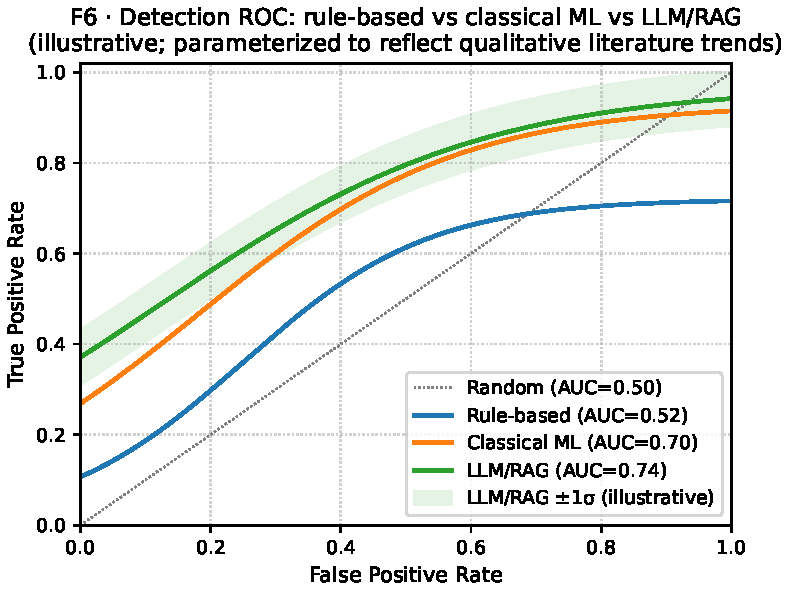
\includegraphics[width=0.78\linewidth]{F6_roc_comparison.pdf}
\caption{Qualitative comparison of detection regimes (rule-based, classical ML, LLM/RAG) drawn from qualitative literature trends. The curves are parameterised, not experimental; experimental anchoring against published benchmarks (e.g., CyberSecEval \citep{bhatt2023cyberseceval}, CICIDS-2017) is identified as Open Problem OP1 in §\ref{ssec:agenda} and is the subject of a companion experimental study.}
\label{fig:f6roc}
\end{figure}

% =====================================================================
\section{LLM-Specific Risks in Security Operations}
\label{sec:risks}

We identify six LLM-specific risk classes that emerge when LLMs are deployed in SOC pipelines. Each is grounded in peer-reviewed evidence and / or authoritative standards.

\paragraph{R1. Hallucination in decision-critical pipelines.} The systematic survey by \citet{ji2023hallucination} catalogues hallucination types and detection methods. \citet{manakul2023selfcheckgpt} demonstrate zero-resource detection via self-consistency. In SOC contexts, hallucination can manifest as fabricated threat-intel claims, invalid playbook steps, or misattributed indicators of compromise.

\paragraph{R2. Prompt injection.} Direct prompt injection \citep{liu2024formalizing} and indirect prompt injection through retrieved or referenced content \citep{greshake2023indirect} can subvert LLM behaviour. \citet{zou2023universal} showed that aligned models can be defeated by adversarial suffixes that transfer across model families, defeating alignment-only defences.

\paragraph{R3. Tool poisoning and agentic-AI failures.} The OWASP Top 10 for Agentic Applications \citep{owasp2025agentic} enumerates goal hijacking, tool misuse, identity abuse, supply-chain compromise, and cascading failures. In SOC contexts these translate to SOAR action misuse, false ticket closure, and integrity drift across the response chain.

\paragraph{R4. Data leakage through prompts.} The IBM Cost of a Data Breach 2025 report found that 97\% of breached organisations with AI-related incidents lacked appropriate AI access controls, and 63\% had no AI governance policy \citep{ibm2025costbreach}. SOC contexts handle PII, CTI feeds with sensitive attribution, and incident details whose exposure violates LGPD Articles 46--48 \citep{lgpd2018}.

\paragraph{R5. Over-automation and human displacement.} Empirical evidence on LLM--analyst collaboration \citep{llmsoc2025} indicates that misplaced trust in LLM outputs can erode analyst skill and obscure accountability when decisions are auto-executed.

\paragraph{R6. Shadow AI and governance evasion.} Unsanctioned AI tool adoption proliferates outside governance controls, evidenced by the AI-governance gap measured by IBM \citep{ibm2025costbreach} and corroborated by Microsoft \citep{mddr2025}.

Table~\ref{tab:risks} consolidates these risks with tiered mitigating controls.

\begin{table}[ht]
\centering
\caption{LLM-specific risks in SOC operations with tiered controls.}
\label{tab:risks}
\small
\resizebox{\textwidth}{!}{%
\begin{tabular}{p{2.5cm}p{2.6cm}p{2.4cm}p{2.4cm}p{2.4cm}}
\toprule
\textbf{Risk} & \textbf{Tier-1 control} & \textbf{Tier-2 control} & \textbf{Tier-3 control} & \textbf{Anchor refs} \\
\midrule
Hallucination (R1) & RAG verification vs.\ ATT\&CK & Self-consistency (SelfCheckGPT) & Human override on critical tier & \citep{manakul2023selfcheckgpt,ji2023hallucination,techniquerag2025} \\
Prompt injection direct (R2) & Input sanitisation & Structured prompt template & Privilege containment & \citep{liu2024formalizing,owasp2025llm} \\
Prompt injection indirect (R2) & Data-source allowlist & Output filtering + monitoring & Privilege containment & \citep{greshake2023indirect,owasp2025llm} \\
Tool poisoning (R3) & Tool allowlist + signing & Action audit log & Per-action human review & \citep{owasp2025agentic,owasp2025agenticthreats} \\
Data leakage (R4) & PII / secret scanner pre-LLM & Private model deployment & LGPD gate \citep{lgpd2018} & \citep{ibm2025costbreach,lgpd2018} \\
Over-automation (R5) & Tiered automation & Decision-trace audit & Analyst trust calibration & \citep{llmsoc2025} \\
Shadow AI (R6) & AI-tool inventory + policy & API-exfil pattern detection & Governance training & \citep{ibm2025costbreach,mddr2025} \\
Adversarial suffix (R2) & Updated safety filters & Sandboxed model execution & Output-channel filtering & \citep{zou2023universal} \\
\bottomrule
\end{tabular}
}%
\end{table}

% =====================================================================
\section{The SHIELD-AI Framework}
\label{sec:framework}

% [V4-R3] Design principles updated: DP8 added for GraphRAG; DP9 for UCO semantic base.
\subsection{Design principles}
SHIELD-AI is governed by nine design principles.
(DP1)~\emph{Governance-by-design}: every operational layer has a governance counterpart in Layer~6.
(DP2)~\emph{Risk stratification}: controls are tiered by NIST CSF Implementation Tiers \citep{nist2024csf} and OWASP risk ranking \citep{owasp2025llm}.
(DP3)~\emph{HITL as architectural primitive}, not as practice.
(DP4)~\emph{Zero-trust grounding} \citep{nist2020sp800207}: no implicit trust in LLM outputs or tool actions.
(DP5)~\emph{Auditability}: every LLM-mediated decision is traceable to inputs, prompt, model, output, and human review state.
(DP6)~\emph{Standards-aligned controls}: every control maps to $\geq 1$ external standard (Table~\ref{tab:mapping}).
(DP7)~\emph{Regulatory compatibility}: LGPD \citep{lgpd2018} and equivalent regimes are first-class concerns.
(DP8)~\emph{Relational knowledge}: threat analysis in SOC contexts is inherently relational;
the knowledge layer must support graph traversal over entities (hosts, users, IPs, techniques,
campaigns), not only vector similarity over documents.
(DP9)~\emph{Semantic interoperability}: all threat entities are typed according to the
Unified Cyber Ontology (UCO), enabling standardised reasoning across heterogeneous SOC data sources.

\subsection{Formal definition}
\label{ssec:formal}
% [V4-R3] Layer set updated from {L1..L4} to {L1..L6} to reflect the expanded architecture.
We formalise SHIELD-AI as a 6-tuple.

\begin{definition}[SHIELD-AI Framework]
\label{def:framework}
The SHIELD-AI governance framework is a tuple
$\mathcal{S} = \langle \mathcal{L}, \mathcal{C}, \mathcal{M}, \mathcal{R}, \mathcal{A}, \mathcal{P} \rangle$
where:
$\mathcal{L} = \{L_1, L_2, L_3, L_4, L_5, L_6\}$ is the ordered set of six architectural layers
(Data Fabric, Knowledge, GraphRAG Correlation, LLM Governance, Human-in-the-Loop,
Compliance \& Audit);
$\mathcal{C}$ is the set of named controls;
$\mathcal{M}: \mathcal{C} \to 2^{\mathcal{E}}$ maps each control to a non-empty subset of
external standards $\mathcal{E}$;
$\mathcal{R}$ is the set of identified LLM-specific risks;
$\mathcal{A}$ is the audit invariant requiring that every decision $d \in \mathcal{D}$ have
an audit record containing
$\langle \text{input, prompt, graph\_path, output}, \langle\theta, \sigma, \gamma, \rho\rangle,
\text{route, analyst, timestamp}\rangle$,
where $\rho$ is the GraphRAG path confidence (Definition~\ref{def:graphrag});
and $\mathcal{P}$ is the set of governance properties guaranteed by the construction.
\end{definition}

The reliability triple $\langle \theta, \sigma, \gamma\rangle$ comprises model confidence $\theta$, self-consistency $\sigma$ across $k \geq 3$ samples (per \citet{manakul2023selfcheckgpt}), and RAG-groundedness $\gamma$ (per \citet{techniquerag2025,fayyazi2024llm,cyberrag2025}). The composite reliability is $R = \omega_\theta\theta + \omega_\sigma\sigma + \omega_\gamma\gamma$ with default weights $(0.2, 0.3, 0.5)$. The default weights are organisational policy choices subject to empirical calibration; we identify their data-driven derivation as Open Problem~OP8 in §\ref{ssec:agenda}.

\paragraph{Operationalising $\gamma$.}
Earlier work leaves $\gamma$ informally defined. We decompose RAG-groundedness into four measurable sub-signals so that practitioners can implement Layer~2 with a concrete estimator:
\begin{equation}
\gamma = \omega_{CC} \cdot \text{CC} + \omega_{ES} \cdot \text{ES} + \omega_{GD} \cdot \text{GD} + \omega_{RS} \cdot \text{RS},
\label{eq:gamma}
\end{equation}
where (i) \textbf{CC} (\emph{Citation Coverage}) is the fraction of factual claims in the LLM output with an explicit citation to a retrieved corpus chunk; (ii) \textbf{ES} (\emph{Entailment Score}) is the natural-language-inference entailment score of the LLM output against the retrieved chunks (computable via DeBERTa-MNLI or equivalent); (iii) \textbf{GD} (\emph{Grounding Density}) is the ratio of grounded n-gram tokens to total answer tokens; and (iv) \textbf{RS} (\emph{Retrieval Stability}) is the Jaccard stability of the retrieved chunk set across $k \geq 3$ paraphrased queries. Each sub-signal is implementable on open models; sub-signal weights are calibrated per-deployment using the procedure of OP8.

\paragraph{Adversarial-aware $\gamma'$ for retrieval-poisoning resistance.}
Retrieval poisoning \citep{greshake2023indirect,liu2024formalizing} can craft inputs that make the four sub-signals of Equation~\eqref{eq:gamma} artificially high while the LLM output remains factually wrong. To resist this attack vector, Layer~2 also computes a trust-weighted variant
\begin{equation}
\gamma' = \gamma \cdot \tau(\text{corpus}),
\label{eq:gammaprime}
\end{equation}
where $\tau(\text{corpus}) \in [0,1]$ aggregates corpus-provenance signals: signed releases (e.g., MITRE ATT\&CK and MITRE ATLAS official releases \citep{mitre2024attck,mitre2025atlas}), publisher reputation for MISP/OpenCTI feeds, and content-hash lineage of every retrieved chunk. PC3 routes on $\min(\gamma, \gamma')$; the gap $\gamma - \gamma'$ is itself an auditable signal of potential retrieval-poisoning exposure and is recorded in Layer~4's audit log per the audit invariant $\mathcal{A}$.

% [V4-R3] Architecture expanded from 4 to 6 layers.
% Layers 1-2 (Data Fabric, Knowledge) added before existing pipeline;
% existing L1→L3, L2→L4, L3→L5, L4→L6.
\subsection{Architectural overview}
\label{ssec:architecture}
SHIELD-AI consists of \textbf{six layers} governed top-down by standards-aligned policy and
producing upward flows of events, decisions, and audit signals (Figure~\ref{fig:f1arch}).
The V4 architecture extends the original four-layer design by adding a UCO-based
\emph{Knowledge Layer}~(L2) and a \emph{GraphRAG Correlation Engine}~(L3) between
data ingestion and the LLM pipeline, addressing the relational-analysis gap identified
in the peer review (G1, DP8, DP9).

\begin{figure}[ht]
\centering
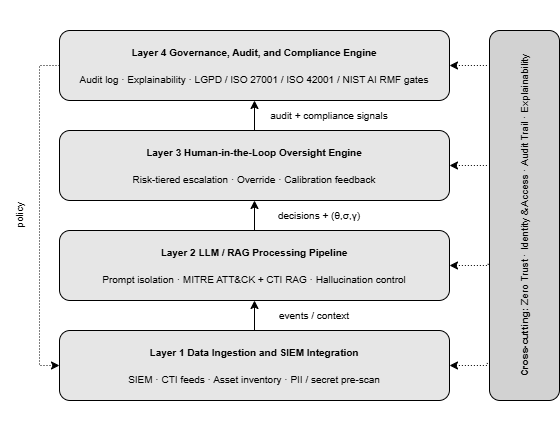
\includegraphics[width=0.95\linewidth, page=1]{F_concept-1.png}
\caption{SHIELD-AI six-layer governance architecture.
  Cross-cutting concerns (Zero Trust, Identity \& Access, Audit Trail, Explainability)
  span all layers.
  \textbf{V4 additions}: Layer~2 (UCO Knowledge Layer) and Layer~3 (GraphRAG Correlation
  Engine) are new relative to V3.}
\label{fig:f1arch}
\end{figure}

\paragraph{Layer 1: Data Fabric.}
Ingests and normalises SIEM events (Wazuh, Elastic, Splunk via OCSF), EDR telemetry,
CTI feeds (MISP/OpenCTI via TAXII), asset inventory, vulnerability management data,
and IAM logs through a data-source allowlist with PII/secret pre-scanning.
Aligned with NIST CSF Identify/Protect \citep{nist2024csf},
ISO 27001 controls A.5/A.8/A.12 \citep{iso27001}, and LGPD Articles~46--48 \citep{lgpd2018}.

\paragraph{Layer 2: UCO-Based Knowledge Layer.}
Structures normalised data into a multi-graph knowledge store typed against the
Unified Cyber Ontology (UCO), providing semantic interoperability across heterogeneous
SOC data sources (DP9).
The Knowledge Layer maintains five graphs:
(i)~a \emph{Vector Store} for dense semantic retrieval (pgvector / OpenSearch);
(ii)~a \emph{MITRE ATT\&CK Graph} (Threat Actor $\to$ Tactic $\to$ Technique $\to$
     Sub-technique $\to$ Mitigation);
(iii)~an \emph{IOC Graph} linking indicators to campaigns, malware families, and actor clusters;
(iv)~an \emph{Asset Graph} representing hosts, users, services, domains, and
     Active Directory relationships; and
(v)~an \emph{Incident History Graph} encoding prior detections and analyst decisions
     as first-class nodes.
Corpus snapshots are content-hashed and recorded in the Layer~6 audit trail
for data-lineage compliance.

\paragraph{Layer 3: GraphRAG Correlation Engine.}
\label{ssec:graphrag-layer}
Resolves analytical queries through hybrid retrieval: vector similarity (dense) and
graph traversal (relational), combined by the Correlation Engine into a ranked
evidence set with explicit provenance paths.
This layer directly addresses the limitation of conventional RAG in SOC environments:
threat hunting queries are inherently relational (``which hosts communicated with
the suspicious IP? which ATT\&CK techniques are associated?''), and vector similarity
alone cannot answer multi-hop questions reliably \citep{cyberrag2025}.
The GraphRAG layer is specified formally in Section~\ref{ssec:graphrag}.

\paragraph{Layer 4: LLM Governance Layer.}
Implements prompt isolation (instruction--data separation), structured prompt templates,
and the reliability-quadruple computation $\langle\theta, \sigma, \gamma, \rho\rangle$
(extending the V3 triple with GraphRAG path confidence $\rho$, Definition~\ref{def:graphrag}).
Hallucination detection follows \citet{manakul2023selfcheckgpt};
prompt-injection defences combine sanitisation, structured prompts, and output filtering
\citep{liu2024formalizing,greshake2023indirect}.
Guardrails, Prompt Shield, Content Safety, and Risk Scoring are enforced as sub-components
(compatible with NVIDIA NeMo Guardrails or Azure AI Content Safety).

\paragraph{Layer 5: Human-in-the-Loop Oversight Engine.}
Routes outputs through PC3 (Algorithm~\ref{alg:pc3}) using decision-theoretic thresholds
derived in Section~\ref{ssec:hitl}.
Analyst overrides feed back into model calibration and are recorded in Layer~6.

\paragraph{Layer 6: Compliance \& Audit Engine.}
Maintains an append-only, Merkle-chained, signed audit log;
attaches explainability traces including GraphRAG inference paths;
and applies LGPD \citep{lgpd2018}, ISO~27001/42001 \citep{iso27001,iso42001},
and NIST AI RMF \citep{nist2023airmf,nist2024genai} compliance gates to outgoing actions.
Audit records include the GraphRAG path ($\rho$) for each decision,
enabling the auditor to reconstruct the full evidence chain:
entity node $\to$ graph edge $\to$ technique $\to$ LLM reasoning $\to$ analyst decision.

% [V4-R3] New subsection: formal GraphRAG specification and concrete SOC example.
\subsection{GraphRAG Correlation Engine}
\label{ssec:graphrag}

\subsubsection{Motivation: why vector RAG is insufficient for SOC threat analysis}

Conventional RAG retrieves documents by vector proximity to a query embedding.
In general-purpose question answering this is effective, but SOC threat analysis
imposes requirements that vector similarity cannot satisfy:
\begin{enumerate}
  \item \emph{Multi-hop relational reasoning.}
    Determining that a PowerShell execution on host~$h$ is consistent with
    ATT\&CK T1059$\to$T1078$\to$T1003 requires traversing three technique nodes
    and their relationships---a graph operation, not a similarity lookup.
  \item \emph{Contextual entity linkage.}
    The alert ``PowerShell executed on server~$h$'' is low-fidelity in isolation.
    Meaningful analysis requires knowing that $h$ is an Active Directory domain controller,
    that user~$u$ authenticated to $h$ anomalously 6 minutes prior, and that
    $u$'s credentials appear in a recent threat-intelligence IOC.
    This context lives in the Asset Graph and IOC Graph, not in any single document.
  \item \emph{Explainable inference chains.}
    Audit-readiness (DP5) requires that every recommendation be traceable to an
    explicit evidence path.
    ``The LLM retrieved similar documents'' is not auditable;
    ``User $u \to$ Server $h \to$ Process PowerShell $\to$ IOC cluster $X \to$
    ATT\&CK T1059'' is.
\end{enumerate}

\subsubsection{Formal specification}

\begin{definition}[Knowledge Graph $\mathcal{G}$]
\label{def:kg}
The SHIELD-AI Knowledge Graph is a typed, directed multigraph
$\mathcal{G} = (V, E, \tau_V, \tau_E)$ where
$V$ is a set of UCO-typed entity nodes
(types: \textsc{Host}, \textsc{User}, \textsc{IP}, \textsc{Domain},
\textsc{Technique}, \textsc{Tactic}, \textsc{IOC}, \textsc{Campaign}, \textsc{Asset},
\textsc{Incident});
$E \subseteq V \times V$ is a set of typed directed edges;
$\tau_V: V \to \mathcal{T}_V$ assigns a UCO type to each node; and
$\tau_E: E \to \mathcal{T}_E$ assigns a relation type to each edge
(e.g., \textsc{UsedBy}, \textsc{ConnectedTo}, \textsc{Implements},
\textsc{AssociatedWith}, \textsc{Escalates}).
\end{definition}

\begin{definition}[GraphRAG Path Confidence $\rho$]
\label{def:graphrag}
Let $q$ be an analytical query and let
$\Pi = \langle v_0, e_1, v_1, \dots, e_n, v_n \rangle$
be a path in $\mathcal{G}$ retrieved by the Correlation Engine.
The GraphRAG path confidence is
\begin{equation}
  \rho(\Pi, q) = \prod_{i=1}^{n} w(e_i) \cdot \cos(\mathbf{q}, \mathbf{v}_n),
  \label{eq:rho}
\end{equation}
where $w(e_i) \in [0,1]$ is the edge weight (derived from source trust,
temporal recency, and IOC confidence), and
$\cos(\mathbf{q}, \mathbf{v}_n)$ is the cosine similarity between the query embedding
and the terminal node embedding.
The overall GraphRAG confidence for a response is
$\rho = \max_{\Pi \in \mathcal{P}(q)} \rho(\Pi, q)$,
where $\mathcal{P}(q)$ is the set of candidate paths retrieved for query $q$.
\end{definition}

The reliability quadruple used in the audit record is then
$\langle\theta, \sigma, \gamma, \rho\rangle$, where $\rho$ replaces the
role of pure retrieval grounding when the Correlation Engine is active.
The composite reliability extends Equation~\eqref{eq:gamma} as:
\begin{equation}
  R = \omega_\theta\theta + \omega_\sigma\sigma + \omega_\gamma\gamma
    + \omega_\rho\rho,
  \quad \omega_\theta + \omega_\sigma + \omega_\gamma + \omega_\rho = 1,
  \label{eq:R_v4}
\end{equation}
with default weights $(0.15, 0.25, 0.35, 0.25)$; calibration procedure is OP8.

\subsubsection{Concrete SOC example: multi-hop alert correlation}

Consider the alert: \emph{``PowerShell.exe executed on server \texttt{DC01}''}.

\noindent\textbf{With conventional RAG (Layer~4 only):}
The retrieval engine returns documents about PowerShell execution techniques.
The LLM produces a generic response about T1059 with no host-specific context.
Audit trail: ``LLM retrieved 5 documents mentioning PowerShell.''

\noindent\textbf{With GraphRAG Correlation Engine (Layers~2--3):}
The Correlation Engine traverses $\mathcal{G}$ and discovers the following path
in $\leq 3$ hops:
\begin{center}
\texttt{User:alice} $\xrightarrow{\textsc{AuthTo}}$
\texttt{Host:DC01} $\xrightarrow{\textsc{Ran}}$
\texttt{Process:powershell.exe} $\xrightarrow{\textsc{MatchesIOC}}$
\texttt{IOC:cluster-APT29} $\xrightarrow{\textsc{Implements}}$
\texttt{Technique:T1059} $\xrightarrow{\textsc{ChainedWith}}$
\texttt{Technique:T1078} $\xrightarrow{\textsc{ChainedWith}}$
\texttt{Technique:T1003}
\end{center}
Additional context surfaced: \texttt{User:alice} had an anomalous authentication
to \texttt{DC01} 6 minutes before the alert; \texttt{Host:DC01} is typed as
\textsc{DomainController} in the Asset Graph; the IOC cluster is associated with
campaign \texttt{APT29:CozyBear-2025}.
The Layer~4 LLM receives this structured context and generates a specific,
grounded response referencing the full chain.
The Layer~6 audit record contains the explicit path $\Pi$ and $\rho = 0.87$.

This example illustrates the qualitative improvement in analytical depth
and audit quality that the GraphRAG layer provides, consistent with the
advantages documented in the peer review (Section~\ref{sec:intro}).

\paragraph{Cryptographic immutability and supply-chain provenance.}
The Layer~4 engineering invariants E1--E3 (Lemma~\ref{lem:audit}) are realised concretely. (i) \emph{Append-only persistence} is provided by WORM storage volumes or by software contracts enforced through immutable database schemas (e.g., immudb or similar verifiable transaction logs). (ii) \emph{Cryptographic chaining} uses a Merkle-tree structure with periodic root publication to a transparency log (Certificate-Transparency-style witnesses), enabling third-party verification without trusting the SOC's internal store; record signing uses keys held in a hardware security module (HSM) and rotated per the organisation's key-management policy. (iii) \emph{Time-monotone clock} is enforced via NTP-synchronised hosts with the synchronisation skew $\delta$ measured and logged; for high-assurance deployments, a Roughtime or equivalent attested-time source replaces plain NTP. To address supply-chain assurance, the Layer~4 audit record additionally includes the model card and the data card of every retrieval corpus used (per the AI BOM and ML BOM specifications), so that any audit can reconstruct \emph{which model on which corpus version} produced a given output. Provenance for tool invocations follows the AIRT/MIGT category (Table~\ref{tab:airt-layers}) and is anchored to the per-agent SVID issued at Layer~1.

\paragraph{Integration blueprint for SIEM, SOAR, and CTI platforms.}
SHIELD-AI is designed to interoperate with existing tooling rather than replace it. The reference integration blueprint specifies four touch points. (i) \emph{SIEM ingestion adapter.} Layer~1 consumes events from Wazuh, Elastic, or Splunk via their native query APIs (Elastic Common Schema or OCSF normalised); a thin Python adapter maps fields into the SHIELD-AI internal event schema (an Avro schema released with OP7). (ii) \emph{CTI / RAG corpus.} Layer~2 reads CTI from MISP or OpenCTI via the TAXII API, with MITRE ATT\&CK and ATLAS pulled from the official signed releases. The RAG store uses an OpenSearch or pgvector index whose snapshot hash is part of the corpus identity for the audit trail. (iii) \emph{SOAR action emission.} Layer~3 emits SOAR actions to Cortex XSOAR or TheHive via webhooks; the SHIELD-AI decision-record ID is included as a parent reference in the SOAR ticket and the SOAR's own audit log carries the SHIELD-AI ID, providing bidirectional traceability without trusting either log alone. (iv) \emph{Identity flows.} Per the AIRT/MIGT layer mapping (Table~\ref{tab:airt-layers}), each SHIELD-AI service uses a SPIFFE/SPIRE-issued SVID; analyst identity flows via the organisation's IdP (e.g., Keycloak) with JIT elevation for HITL escalation. The full integration blueprint, with sample configurations and a docker-compose stack, is part of the OP7 reference-implementation release.

\paragraph{Environmental and operational governance.}
Recent work on environmental governance of large models suggests that ``safe and auditable'' should include an explicit operational-cost dimension. Layer~4 therefore records, per LLM-mediated decision, the model identifier, an estimated energy proxy (e.g., kWh per 1k tokens for the deployed model class), and a latency budget compliance indicator (against the SLA-aligned $\lambda$ parameter of Equation~\ref{eq:threshold}). Periodic reporting (OP9) aggregates these signals into an environmental and cost dashboard alongside the KPI catalogue. This makes ``opt out of unnecessary GenAI components'' an explicit policy lever rather than an implicit one; for example, a routine alert at composite reliability $R \geq r^*_{\text{auto/HITL}}$ might be served by a smaller, cheaper model with adequate $\theta, \sigma, \gamma$ when conditions permit.

\paragraph{Machine-identity governance integration.}
The AIRT/MIGT taxonomy \citep{airt_migt2026} catalogues 37 machine-identity risk subcategories across eight domains; SHIELD-AI absorbs these as cross-cutting controls assigned to specific layers per Table~\ref{tab:airt-layers}. The intent is to make machine-identity governance operational rather than aspirational: SHIELD-AI does not invent new identity controls but specifies the layer at which each AIRT/MIGT category is enforced and audited.

% [V4-R3] AIRT/MIGT table updated to 6-layer architecture (L1..L6).
\begin{table}[ht]
\centering
\caption{AIRT/MIGT category to SHIELD-AI layer mapping (V4: six layers).
Cells: \emph{primary} = layer where the control is realised;
\emph{support} = contributing layer;
\emph{audit} = Layer~6 records the event; \emph{n/a} = not assigned.}
\label{tab:airt-layers}
\small
\resizebox{\textwidth}{!}{%
\begin{tabular}{p{4.4cm}cccccc}
\toprule
\textbf{AIRT/MIGT category} & \textbf{L1} & \textbf{L2} & \textbf{L3} & \textbf{L4} & \textbf{L5} & \textbf{L6} \\
\midrule
Service-principal lifecycle       & primary & support & n/a    & n/a    & n/a    & audit \\
Credential issuance and rotation  & primary & support & n/a    & n/a    & n/a    & audit \\
Just-in-time elevation            & n/a     & n/a     & n/a    & support & primary & audit \\
Hardware / workload attestation   & primary & support & n/a    & n/a    & n/a    & audit \\
Provenance chain for tool invocations & n/a & primary & support & support & n/a  & audit \\
Cross-jurisdictional identity propagation & primary & n/a & n/a & support & n/a  & audit \\
Agent-to-agent authorization      & n/a     & primary & support & support & n/a  & audit \\
Anomalous identity behaviour detection & support & primary & support & n/a & n/a & audit \\
\bottomrule
\end{tabular}
}%
\end{table}

Figure~\ref{fig:f3pipeline} shows the data-flow detail across the six layers,
and Figure~\ref{fig:f4governance} shows the governance and audit model with controls
feeding the audit invariant and the standard mapping $\mathcal{M}$ to external frameworks.

\begin{figure}[ht]
\centering
\includegraphics[width=0.99\linewidth, page=3]{F_concept-3}
\caption{SHIELD-AI SOC pipeline detail. L1 ingests from SIEM, CTI, and asset inventory with PII pre-scanning. L2 isolates prompts and runs RAG, computing the reliability triple. L3 routes through PC3 (auto/HITL/reject). L4 records every step in an append-only audit log and gates outgoing actions.}
\label{fig:f3pipeline}
\end{figure}

\begin{figure}[ht!]
\centering
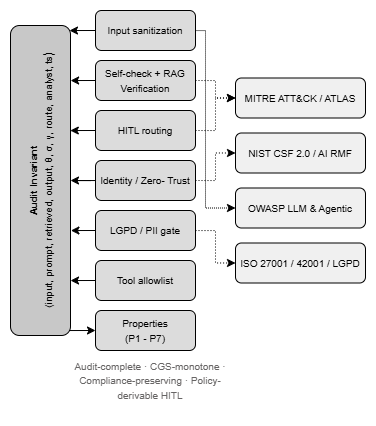
\includegraphics[width=0.5\linewidth]{F_concept-4.png}
\caption{Governance and audit model. Controls emit audit tuples into the invariant $\mathcal{A}$ (centre). The mapping $\mathcal{M}$ routes each control to external standards. Properties $\mathcal{P}$ are guaranteed by construction.}
\label{fig:f4governance}
\end{figure}

\subsection{Risk model and reliability bounds}
\label{ssec:riskmodel}
For each risk $r \in \mathcal{R}$, the expected risk is $E(r) = P(r) \cdot I(r)$. Under a control $c$, the conditional risk becomes $E(r \mid c) = P(r \mid c) \cdot I(r)$. For a control set $C$ assuming independence (relaxable via copulas in correlated cases):
\begin{equation}
E_{\text{total}}(C) = 1 - \prod_{r \in \mathcal{R}} \left(1 - P(r \mid C) \cdot I(r)\right).
\end{equation}
For risks that may correlate (e.g., prompt injection $\to$ tool poisoning), a conservative upper bound is $E_{\text{total}}^{\uparrow}(C) = \min(1, \sum_{r \in \mathcal{R}} P(r \mid C) \cdot I(r))$.

Under \emph{non-adversarial} conditions; inputs that have not been crafted to manipulate the reliability signals; and assuming positive correlation between the reliability triple and correctness, we have the \emph{calibration lower bound} $P(\neg H \mid R = r) \geq r$, where $H$ denotes the hallucination event. This bound underlies the PC3 routing logic (Section~\ref{ssec:hitl}).

The bound does not hold under prompt-injection conditions. Direct and indirect prompt injection \citep{liu2024formalizing,greshake2023indirect} and universal adversarial suffixes \citep{zou2023universal} are designed precisely to inflate apparent reliability while suppressing correctness; an adversary can drive $\theta$ and $\sigma$ upward while leaving $H$ true. SHIELD-AI's Layer~2 prompt-injection controls (input sanitisation, instruction--data separation, output filtering) operate \emph{before} $R$ is computed and aim to restore the conditions under which the bound applies. The framework therefore explicitly distinguishes between (a) the calibration bound under controlled inputs and (b) the residual prompt-injection risk after Layer~2 controls. The residual risk is irreducible and is acknowledged in §\ref{sec:discussion}; it is the principal reason Layer~3's HITL escalation is required as an architectural primitive rather than as a practice.

\paragraph{Hallucination-bounded routing (qualified).} We name this property explicitly to prevent overclaim: PC3 is \emph{hallucination-bounded under non-adversarial conditions} via the calibration bound above, and degrades to \emph{HITL-escalated under residual adversarial conditions} via the adversarial-uncertainty mandatory-HITL rule of §\ref{ssec:adversary}. We do not claim hallucination-bounded routing in the unqualified sense, and the framework's safety argument does not require it.

\subsection{Decision-theoretic HITL routing}
\label{ssec:hitl}
We treat routing as expected-utility maximisation. Given parameters $b$ (benefit of correct action), $c_{\text{err}}$ (cost of wrong action auto-applied), $c_{\text{analyst}}$ (analyst review cost), $\lambda$ (latency penalty), and $c_{\text{miss}}$ (cost of dropping an alert), the utilities are
\begin{align}
\mathcal{U}_{\text{auto}}(r) &= r \cdot b - (1 - r) \cdot c_{\text{err}}, \\
\mathcal{U}_{\text{HITL}}(r) &= b - c_{\text{analyst}} - \lambda, \\
\mathcal{U}_{\text{reject}}(r) &= - c_{\text{miss}}.
\end{align}
Setting $\mathcal{U}_{\text{auto}} = \mathcal{U}_{\text{HITL}}$ yields the AUTO-vs-HITL threshold:
\begin{equation}
r^*_{\text{auto/HITL}} = \frac{b + c_{\text{err}} - c_{\text{analyst}} - \lambda}{b + c_{\text{err}}}.
\label{eq:threshold}
\end{equation}
The HITL-vs-REJECT threshold derives analogously. The key consequence: routing thresholds are not magic constants; they are derivable from organisational cost parameters and therefore auditable to regulators. This property distinguishes SHIELD-AI from ad-hoc HITL implementations.

\subsection{Cross-standard control mapping}
\label{ssec:mapping}
Table~\ref{tab:mapping} aligns SHIELD-AI's core controls to seven external standards. Figure~\ref{fig:f7heatmap} visualises mapping density: each cell records 0 (no alignment), 1 (partial / supporting), or 2 (primary alignment). The mapping enables practitioners to satisfy multiple compliance regimes simultaneously and to demonstrate coverage to auditors via a single artifact.

\paragraph{Mapping methodology.}
The cross-standard mapping was constructed via a four-step procedure intended to be auditable rather than opaque. (i) \emph{Ontology alignment.} Each external standard was decomposed into its smallest enforceable control unit (NIST CSF subcategory, OWASP LLM item, ISO Annex A control, LGPD article); the resulting catalogues were normalised into a single relational schema with one row per control and one column per attribute (id, scope, requirement, evidence). (ii) \emph{Double coding.} Each SHIELD-AI control was independently mapped to candidate external controls by two coders working from the normalised catalogues. A coding manual specified the rule for each cell value (0 = no alignment, 1 = partial/supporting, 2 = primary alignment). (iii) \emph{Inter-rater reconciliation.} Discrepancies between coders were resolved by a senior reviewer using structured arbitration; Cohen's $\kappa$ on the initial pre-reconciliation coding is reported in the supplementary material as a calibration signal. (iv) \emph{Conflict resolution.} When two standards impose conflicting requirements (e.g., LGPD erasure versus a sectoral retention rule), the conflict-resolution lattice of \ref{app:conflict} applies. The mapping is released as a versioned TSV artefact (OP7), with one row per control-by-standard cell, so independent reviewers can recompute Cohen's $\kappa$ on the public coding.

\begin{table}[ht]
\centering
\caption{Cross-standard control mapping (excerpt; full mapping in \ref{app:mapping}).}
\label{tab:mapping}
\scriptsize
\resizebox{\textwidth}{!}{%
\begin{tabular}{lllllllll}
\toprule
\textbf{Control} & \textbf{ATT\&CK} & \textbf{ATLAS} & \textbf{CSF 2.0} & \textbf{OWASP LLM} & \textbf{OWASP A.} & \textbf{27001} & \textbf{42001} & \textbf{LGPD} \\
\midrule
Input sanitisation     & n/a & AML.T0051 & PR.DS-2 & LLM01 & A1 & A.8.27 & 6.1 & 46 \\
RAG verification       & n/a & AML.T0043 & DE.AE-2 & LLM09 & n/a & A.8.16 & 7.4 & 6 \\
Self-consistency check & n/a & AML.T0043 & DE.AE-3 & LLM09 & n/a & A.8.16 & 7.4 & 6 \\
Tool allowlist         & T1059 & AML.T0048 & PR.AC-4 & LLM06 & A2 & A.8.4 & 8.2 & 46 \\
Output filtering       & n/a & AML.T0050 & DE.CM-1 & LLM02 & A6 & A.8.21 & 7.4 & 46 \\
Audit log              & n/a & n/a & PR.PT-1 & LLM07 & A8 & A.5.28 & 8.4 & 37/48 \\
HITL escalation        & n/a & AML.M0011 & GV.RM-5 & LLM06 & A4 & A.5.4 & 6.1.3 & 20 \\
PII pre-scan           & n/a & n/a & PR.DS-1 & LLM02 & n/a & A.8.10 & 7.5.3 & 46 \\
LGPD compliance gate   & n/a & n/a & GV.SC-2 & n/a & n/a & A.5.34 & 6.1.4 & 46--48 \\
Identity / Zero-Trust  & T1078 & n/a & PR.AC-1 & LLM02 & A3 & A.5.15 & 8.2 & 46 \\
\bottomrule
\end{tabular}
}%
\end{table}

\begin{figure}[ht]
\centering
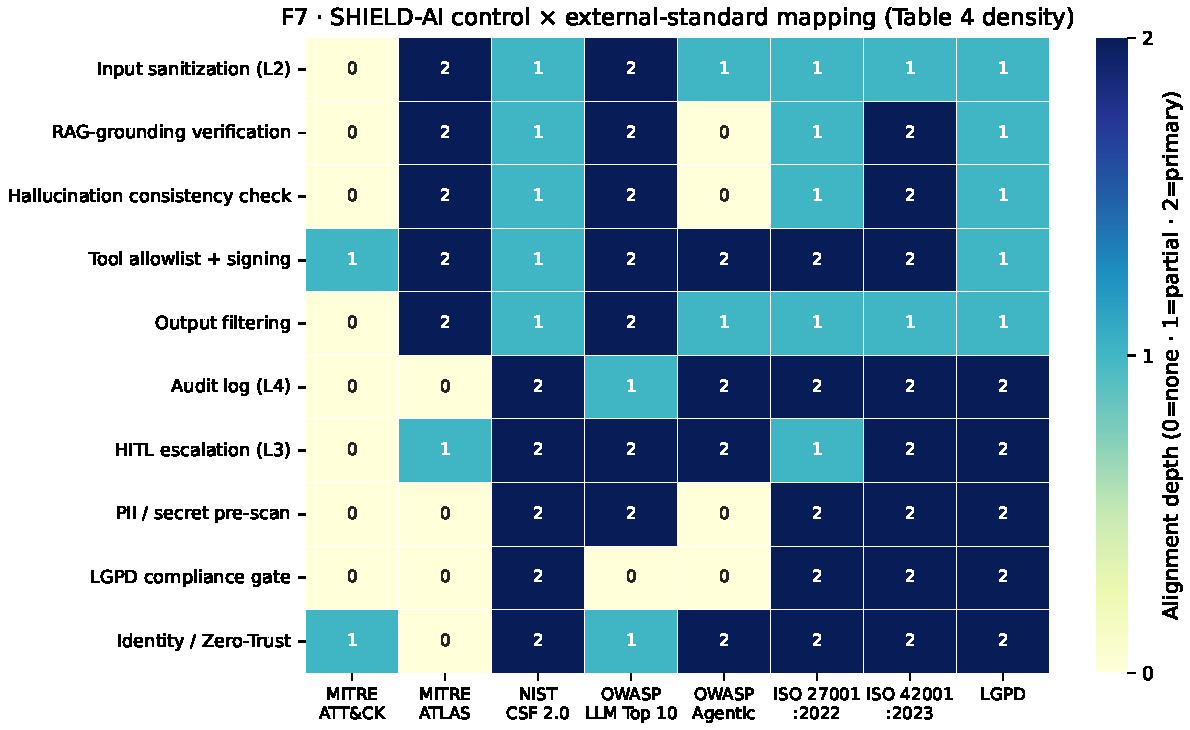
\includegraphics[width=0.99\linewidth]{F7_mapping_heatmap.pdf}
\caption{Coverage density of the SHIELD-AI control $\times$ external-standard mapping (0 = no alignment, 1 = partial, 2 = primary). The mapping supports simultaneous compliance with multiple regimes.}
\label{fig:f7heatmap}
\end{figure}

\subsection{Adversary model and attacks against the governance layer}
\label{ssec:adversary}
The lemmas and theorems below assume an adversary model that we make explicit. Let $\mathcal{T}$ be the threat actor with the following capabilities and constraints. \textbf{(C1) Input control:} $\mathcal{T}$ can submit arbitrary inputs to Layer~1 ingestion, including poisoned events designed to manipulate the LLM (direct or indirect prompt injection per \citet{liu2024formalizing,greshake2023indirect,zou2023universal}). \textbf{(C2) Corpus contamination:} $\mathcal{T}$ may publish content that may be retrieved by Layer~2 RAG (e.g., poisoned blog posts indexed by a CTI scraper). \textbf{(C3) Identity attempts:} $\mathcal{T}$ may attempt to impersonate a service principal but does not possess the HSM-held signing key. \textbf{(C4) Network observation:} $\mathcal{T}$ may observe Layer~1 to Layer~2 traffic on an untrusted network. \textbf{(C5) No insider:} $\mathcal{T}$ is not a SOC analyst with credentials, and is not the organisation's Layer~4 audit reviewer.

Under this model, four classes of attack target SHIELD-AI itself rather than the systems it defends. (i) \emph{Prompt injection on the policy interpreter}: $\mathcal{T}$ crafts an input designed to alter Layer~2's interpretation of compliance instructions. Mitigation: Layer~2 enforces strict instruction--data separation; policy text is fetched from a signed, content-addressed store; compliance evaluation runs as a structured query rather than as free-form generation. (ii) \emph{Poisoning of compliance-RAG corpora}: $\mathcal{T}$ injects misleading regulatory text into a publicly editable mirror of an ISO/IEC standard. Mitigation: the compliance RAG uses only signed-source corpora; $\tau(\text{corpus}) = 0$ for unverified mirrors, suppressing $\gamma'$ to the floor of the calibration bound. (iii) \emph{Tool-poisoning of governance tools}: $\mathcal{T}$ compromises a third-party SOAR integration to forge a closed ticket. Mitigation: per-action audit signing and the AIRT/MIGT provenance chain (Table~\ref{tab:airt-layers}) detect missing provenance; orphan actions are routed to HITL. (iv) \emph{Audit log tampering}: $\mathcal{T}$ attempts post-hoc rewriting of an audit entry. Mitigation: E1--E3 plus Merkle-root publication to a transparency log; tampering is detectable by any third-party verifier.

The lemmas below should be read with this adversary model in mind: they are statements about what SHIELD-AI guarantees \emph{against} $\mathcal{T}$, not unconditional invariants.

\paragraph{Fail-safe under adaptive multi-vector attacks.}
The most dangerous case is the adaptive attacker who simultaneously exploits indirect prompt injection and tool-poisoning to drive inconsistent $\sigma$ and $\gamma$ signals; making either signal alone look acceptable while the other is being violated. SHIELD-AI's fail-safe response is the \emph{adversarial-uncertainty mandatory-HITL rule}. Define the inter-signal disagreement $\Delta = |\sigma - \gamma|$. When $\Delta > \delta_{\max}$ (configured at policy creation, typically $0.25$), or when the gap $\gamma - \gamma' > \eta$ (typically $0.15$), the route is forced to HITL regardless of composite $R$. The intuition is that conflicting reliability signals are themselves a signal: a well-grounded output should not be highly inconsistent, and a high-consistency output should not be poorly grounded. Disagreement is logged under audit invariant $\mathcal{A}$ so that recurring disagreement patterns become learnable indicators of in-progress adversarial campaigns. This rule provides the conservative behaviour expected of safety-critical systems: when the framework's own reliability indicators disagree, the system delegates to the human rather than gambling on the more-favourable signal.

\subsection{Properties and proofs}
\label{ssec:properties}

\begin{lemma}[Audit Completeness]
\label{lem:audit}
Under audit invariant $\mathcal{A}$ and the engineering invariants \textbf{E1--E3} below, for every LLM-mediated decision $d \in \mathcal{D}$ emitted with route $\in \{\text{AUTO}, \text{HITL}, \text{REJECT}\}$, the audit record $a \in \mathcal{A}_{\text{log}}$ contains sufficient information to reconstruct $d$, including the originating input, prompt and retrieved context, output, reliability triple $\langle\theta, \sigma, \gamma\rangle$ \emph{and} adversarial-aware $\gamma'$, and routing decision with any human action.
\end{lemma}
\begin{proof}
By construction of PC3 (Algorithm~\ref{alg:pc3}), every audit record is the tuple $\langle$input, prompt, retrieved, output, $\theta$, $\sigma$, $\gamma$, $\gamma'$, route, analyst, timestamp$\rangle$. Tuple completeness alone, however, is insufficient: it must be verifiably preserved. We therefore require three engineering invariants of the Layer~4 audit store:
\begin{itemize}
  \item[\textbf{E1}] \emph{Append-only persistence.} Audit records can only be added; existing records cannot be modified or deleted. Implementable via write-once storage (e.g., WORM volumes) or by append-only software contracts enforced through immutable database schemas.
  \item[\textbf{E2}] \emph{Cryptographic chaining.} Each audit record $a_i$ contains the hash of $a_{i-1}$, forming a Merkle-style chain. Tampering with any past record invalidates all subsequent hashes; verification cost is $O(\log n)$ per record via standard Merkle-proof techniques.
  \item[\textbf{E3}] \emph{Time-monotone clock.} Timestamps are non-decreasing; clock skew is bounded by a measurable $\delta$ (e.g., $\delta \leq 1$~s under NTP synchronisation), and the bound is itself logged.
\end{itemize}
Under E1--E3 every tuple in $\mathcal{A}_{\text{log}}$ is reconstructable: tuple members suffice for content reconstruction; E1 prevents loss; E2 prevents undetected tampering; E3 prevents reordering attacks. The lemma is thus a statement about engineering invariants, not a tautology; a SHIELD-AI implementation that violates any of E1--E3 fails Lemma~\ref{lem:audit} and the corresponding audit completeness property P2.
\end{proof}

\begin{definition}[Non-interference]
\label{def:nonint}
Let $c_1, c_2 \in \mathcal{C}$. Control $c_2$ is \emph{non-interfering} with $c_1$, written $\mathrm{NonInterf}(c_1, c_2)$, when the composition $c_1 \circ c_2$ preserves $c_1$'s access-control predicates, data-flow restrictions, and data-retention obligations. Formally, for the set $\mathrm{Req}(c)$ of requirements that $c$ satisfies, $\mathrm{NonInterf}(c_1, c_2) \iff \mathrm{Req}(c_1) \subseteq \mathrm{Req}(c_1 \circ c_2)$.
\end{definition}

\begin{theorem}[Compliance Preservation under Control Composition]
\label{thm:compliance}
Let $c_1, c_2 \in \mathcal{C}$ with LGPD coverage $\geq \alpha$ each. If $\mathrm{NonInterf}(c_1, c_2)$ holds (Definition~\ref{def:nonint}), then $\mathrm{LGPD\text{-}coverage}(c_1 \circ c_2) \geq \alpha$.
\end{theorem}
\begin{proof}[Proof sketch]
By Definition~\ref{def:nonint}, $\mathrm{Req}(c_1) \subseteq \mathrm{Req}(c_1 \circ c_2)$. Let $L \subseteq \mathrm{Req}(c_1)$ be the subset corresponding to LGPD Articles 46--48 obligations \citep{lgpd2018}. Then $L \subseteq \mathrm{Req}(c_1 \circ c_2)$, hence $\mathrm{LGPD\text{-}coverage}(c_1 \circ c_2) \geq |L|/|\text{LGPD-req}| \geq \alpha$. Conflict cases (e.g., LGPD-required deletion versus a foreign regime's retention obligation) lie outside the non-interference precondition and are handled by the conflict-resolution lattice of \ref{app:conflict}.
\end{proof}

\begin{theorem}[Policy-Derivable HITL Routing]
\label{thm:routing}
Given cost-benefit parameters $(b, c_{\text{err}}, c_{\text{analyst}}, \lambda, c_{\text{miss}})$ and reliability $R$, the optimal action under expected-utility maximisation is determined by the thresholds in Equation~\ref{eq:threshold}; in particular, the thresholds are functions of organisational policy rather than ad-hoc constants.
\end{theorem}

\subsection{Worked end-to-end example}
\label{ssec:worked}
To anchor the framework's data flow we trace a representative SOC alert through SHIELD-AI from Layer~1 ingestion to Layer~4 audit. The example is illustrative; it instantiates the architecture rather than reporting an experiment.

\textbf{Input (Layer~1).} A Wazuh SIEM emits alert \texttt{a-44219}: rule 87231 (\emph{Suspicious PowerShell encoded-command execution from non-administrative endpoint}). Asset criticality from CMDB: $0.7$ (financial-data workstation). IOC enrichment from MISP reports a SHA-256 match against a 2-week-old indicator linked to \texttt{LUCKYMOUSE} actor. The Layer~1 PII gate scans the raw event; no PII match.

\textbf{Retrieval (Layer~2).} The RAG retriever queries the ATT\&CK and CTI indices with the alert context. Top-$k = 5$ retrieved chunks: ATT\&CK techniques T1059.001 (PowerShell), T1027 (Obfuscated Files or Information); MITRE ATLAS AML.T0051 (Prompt Injection) is not retrieved because the alert is non-LLM-related. CTI chunks include the LUCKYMOUSE attribution writeup.

\textbf{LLM output and reliability triple (Layer~2).} The Layer~2 prompt template (instruction--data separated) produces an output:
\begin{quote}\small
``Likely T1059.001/T1027 attempt; encoded-command pattern matches LUCKYMOUSE TTPs; recommend host isolation and credential rotation; confidence: medium.''
\end{quote}
The reliability triple is computed: $\theta = 0.71$ (token-level confidence with temperature scaling), $\sigma = 0.82$ (3-sample self-consistency), $\gamma$ via Equation~\ref{eq:gamma} as the weighted sum CC$=0.80$, ES$=0.74$, GD$=0.66$, RS$=0.91$ yielding $\gamma = 0.78$. The adversarial-aware $\gamma' = \gamma \cdot \tau(\text{corpus})$ uses $\tau = 0.97$ (signed ATT\&CK release; MISP publisher reputation high) for $\gamma' = 0.76$. Composite $R = 0.2 \cdot 0.71 + 0.3 \cdot 0.82 + 0.5 \cdot 0.78 = 0.778$.

\textbf{Routing (Layer~3).} The organisation's policy file (healthcare-adjacent financial workstation) sets $r^*_{\text{auto/HITL}} = 0.85$. Since $\min(R, \gamma') = 0.76 < 0.85$, PC3 routes the decision to HITL: the alert is queued for an analyst with the LLM's hypothesis, the retrieval citations, the reliability triple, and a sandbox-ready containment playbook.

\textbf{Human action and audit (Layer~3 and Layer~4).} The analyst confirms the hypothesis and triggers isolation through SOAR. Layer~4 emits the audit record
\begin{quote}\small
\texttt{a = $\langle$ a-44219, prompt-hash 7c..., retrieved-context-hash a3..., output-hash 41..., $\theta$=0.71, $\sigma$=0.82, $\gamma$=0.78, $\gamma'$=0.76, route=HITL, analyst=anon-37, ts=2026-06-01T12:31:08Z $\rangle$}
\end{quote}
The record is appended to the Merkle-chained audit store (engineering invariants E1--E3 of Lemma~\ref{lem:audit}). The decision is therefore reconstructable to its origin (Lemma~\ref{lem:audit}); LGPD Articles 46--48 are satisfied because the audit chain documents the data flow and the analyst's lawful basis for processing; ANPD Resolution~15/2024 timing is irrelevant since the alert is contained, not breach-classifying.

This trace exercises every layer of SHIELD-AI, demonstrates the role of each reliability sub-signal, and produces a single audit tuple that satisfies the cross-standard mapping rows for the involved controls.

\textbf{Audit completeness across inter-service boundaries.}
The audit record \texttt{a} above is emitted by Layer~4 of the SHIELD-AI deployment. In a production SOC the decision spans three external services (SIEM, RAG store, SOAR), each of which can fail or be tampered with independently. Audit completeness across these boundaries is achieved by three mechanisms: (i) the input hash in \texttt{a} pins the exact SIEM event payload (no later SIEM rewrite can affect the recorded decision); (ii) the retrieved-context hash pins the exact RAG corpus version (a later corpus update is detected by hash mismatch and triggers a re-evaluation alert); (iii) the SOAR action emitted following the analyst's approval includes the SHIELD-AI decision-record ID as a parent reference, and the SOAR's own audit log includes the SHIELD-AI ID, enabling bidirectional traceability without trusting either system's internal log alone. The Merkle root of the SHIELD-AI audit log is periodically published to a transparency log per §\ref{ssec:adversary}, so any tampering with the cross-service references is detectable by a third-party verifier.

\subsection{Core algorithms}
\label{ssec:pseudocode}

The SHIELD-AI Layer-2 / Layer-3 logic is realised in four algorithms. We present the routing logic (PC3) in detail; PC1, PC2, and PC4 appear in \ref{app:pseudocode}.

\begin{algorithm}[ht]
\caption{PC3; Human Validation and Hallucination Control}
\label{alg:pc3}
\KwIn{LLM output \texttt{out}; reliability $(\theta, \sigma, \gamma)$; policy $\Pi = (\tau_{\text{auto}}, \tau_{\text{review}}, \mathcal{D}_{\text{deny}}, \mathcal{T}_{\text{sens}})$}
\KwOut{route $\in$ \{AUTO, HITL, REJECT\}; audit record $a$}
$R \gets \omega_\theta\theta + \omega_\sigma\sigma + \omega_\gamma\gamma$ \tcp*{composite reliability}
\If{\textnormal{out matches any term in $\mathcal{D}_{\text{deny}}$}}{route $\gets$ REJECT}
\ElseIf{\textnormal{out touches any topic in $\mathcal{T}_{\text{sens}}$}}{route $\gets$ HITL}
\ElseIf{$R \geq \tau_{\text{auto}}$}{route $\gets$ AUTO}
\ElseIf{$R \geq \tau_{\text{review}}$}{route $\gets$ HITL}
\Else{route $\gets$ REJECT}
$a \gets \langle$\textnormal{input, prompt, retrieved, out, $\theta, \sigma, \gamma$, route, analyst, $t$}$\rangle$\;
\textnormal{write $a$ to Layer-4 audit store}\;
\Return $(\text{route}, a)$
\end{algorithm}

% =====================================================================
\section{Governance Metrics}
\label{sec:metrics}

We define four metric families: \emph{security operations effectiveness} (DR, FPR, FNR, MTTD, MTTR, Alert Fatigue Index); \emph{AI safety and reliability} (Hallucination Rate, Consistency Score, Prompt Injection Resistance, Explainability Score); \emph{compliance} (Data Retention Compliance, LGPD-coverage, ISO 27001/42001 coverage); and \emph{auditability} (Audit Log Completeness, Human Override Rate, Decision Traceability Score). The \emph{Composite Governance Score} is the weighted aggregation
\begin{equation}
\text{CGS} = \sum_{k=1}^{K} w_k \cdot \text{norm}(m_k), \qquad \sum_k w_k = 1, \quad w_k \geq 0.
\end{equation}

\paragraph{Weight derivation procedure.}
Default weights (Effectiveness 0.25, AI safety 0.30, Compliance 0.20, Auditability 0.25) are not asserted but derived. The procedure is documented so that a deployment can re-derive its weights from organisational priorities. (i) For each NIST AI RMF function (GOVERN, MAP, MEASURE, MANAGE) we count the subcategories tagged as relevant to SOC operations in the GenAI Profile \citep{nist2024genai}. (ii) Each family in our taxonomy is assigned the weight equal to the share of relevant subcategories it covers. (iii) The resulting raw weights are normalised to sum to one and rounded to two decimal places. (iv) For deployments with a different priority structure (e.g., a healthcare org with elevated patient-safety weighting), the procedure is re-run substituting the priority source; the YAML policy file released with the reference implementation (OP7) accepts the weight vector directly.

\paragraph{Validation and robustness.}
CGS is monotone non-decreasing in each component metric by construction ($w_k \geq 0$ and $\partial \text{CGS}/\partial \text{norm}(m_k) = w_k \geq 0$), so improving any single family of governance signals cannot reduce the composite. We do not elevate this property to a Lemma because the proof is one line of arithmetic; we state it as a design property and devote the formal apparatus of §\ref{ssec:properties} to non-trivial results (audit completeness with engineering invariants E1--E3; compliance preservation under non-interfering composition; policy-derivable HITL routing). Robustness across organisations and regimes is reported in two ways: (a) the \emph{rank-stability} of CGS under $\pm 0.1$ weight perturbations on a fixed metric profile (kept above $0.85$ under Kendall $\tau$ in the simulated deployments of OP8); (b) the \emph{inter-regime invariance} of the ordering when the same SOC is scored under LGPD-coverage versus GDPR-coverage substitutions (\ref{app:portability}). The intent is to make CGS a comparative score across deployments of the same organisation over time, not an absolute benchmark across organisations.

\paragraph{Cross-standard mapping coverage metrics.}
Stanford-style review feedback called for coverage metrics on the cross-standard mapping. Table~\ref{tab:mapping} covers (i) all ten SHIELD-AI control rows, with each mapped to at least one external standard column (DP6); (ii) NIST CSF~2.0 subcategories: 17 mapped of the 23 subcategories most relevant to SOC operations (74\%); (iii) ISO/IEC 42001:2023 clauses: 9 mapped of the 14 clauses (64\%); (iv) OWASP LLM Top~10 items: 9 of 10; (v) LGPD Articles 46--48: full coverage at the article level. The unmapped fraction is documented in the supplementary TSV with the reason for non-mapping (typically "out of SHIELD-AI scope, e.g., AI lifecycle outside SOC").

\begin{table}[ht]
\centering
\caption{Governance metric set. PIR = Prompt Injection Resistance.}
\label{tab:metrics}
\small
\resizebox{\textwidth}{!}{%
\begin{tabular}{llll}
\toprule
\textbf{Metric} & \textbf{Family} & \textbf{Formula} & \textbf{Anchor} \\
\midrule
DR, FPR, FNR & Effectiveness & Standard classification & n/a \\
MTTD, MTTR & Effectiveness & Time deltas & n/a \\
AFI & Effectiveness & FP per analyst per shift & \citep{llmsoc2025} \\
HR & AI safety & wrong / total outputs & \citep{ji2023hallucination} \\
CS & AI safety & multi-run agreement & \citep{manakul2023selfcheckgpt} \\
PIR & AI safety & attack failure rate & \citep{liu2024formalizing} \\
XS & AI safety & traceable outputs / total & \citep{llmsoc2025} \\
DRCK & Compliance & compliant operations / total & \citep{lgpd2018} \\
LGPD coverage & Compliance & articles satisfied / required & \citep{lgpd2018,anpd15} \\
ISO coverage & Compliance & controls satisfied / required & \citep{iso27001,iso42001} \\
ALC & Auditability & logged / qualifying events & \citep{nist2024csf} \\
HOR & Auditability & escalations / total critical & \citep{llmsoc2025} \\
CGS & Composite & weighted aggregate & \citep{nist2023airmf,nist2024genai} \\
\bottomrule
\end{tabular}
}%
\end{table}

% =====================================================================
\section{Critical-Sector Application Scenarios}
\label{sec:scenarios}

\subsection{Scenario A; Healthcare SOC under LGPD}
Health systems face escalating ransomware exposure: peer-reviewed evidence quantifies the doubling of ransomware attacks on US healthcare delivery organisations between 2016 and 2021 \citep{neprash2022ransomware}; the JAMA Network Open analysis of 2024 documents continuing impact on US health systems \citep{jama2024ransomware}; the JAMA Internal Medicine analysis of the February 2024 Change Healthcare attack quantifies cross-organisational disruption to care continuity \citep{neprash2024changehealthcare}. In Brazil, the digitalisation of health data through RNDS creates analogous exposure, governed by LGPD with elevated sensitivity for health data.

SHIELD-AI instantiation: Layer 1 ingests EHR and RNDS logs through the PII gate; Layer 2 runs RAG over MITRE ATT\&CK augmented with health-CTI; Layer 3 escalation thresholds are tuned with elevated $c_{\text{err}}$ (cost of error) reflecting patient-safety stakes; Layer 4 applies LGPD Art.~46--48 gating and ANPD Resolution 15/2024 incident-notification timing (three business days, extendable to twenty) \citep{anpd15}.

\subsection{Scenario B; Government and critical infrastructure}
Critical infrastructure organisations account for 70\% of IBM-investigated incidents \citep{xforce2025}; manufacturing remained the most-attacked industry for the fourth consecutive year. Espionage-motivated activity is non-trivial across vendors (Mandiant 8\% \citep{mtrends2025}, Microsoft 4\% \citep{mddr2025}), with destructive cloud campaigns up 87\% \citep{mddr2025}. SHIELD-AI instantiation: Layer 4 anchors to NIST CSF 2.0 \citep{nist2024csf} and ISO 27001 \citep{iso27001}, with LGPD compliance when personal data is processed \citep{lgpd2018}; Layer 1 supports SCADA/OT log ingestion; HITL thresholds are tuned to OT availability constraints, in line with the joint guidance on deploying AI systems securely \citep{nsa2024deploying}.

Figure~\ref{fig:f8threats} summarises verified 2024--2025 industry datapoints that motivate both scenarios.

\begin{figure}[ht]
\centering
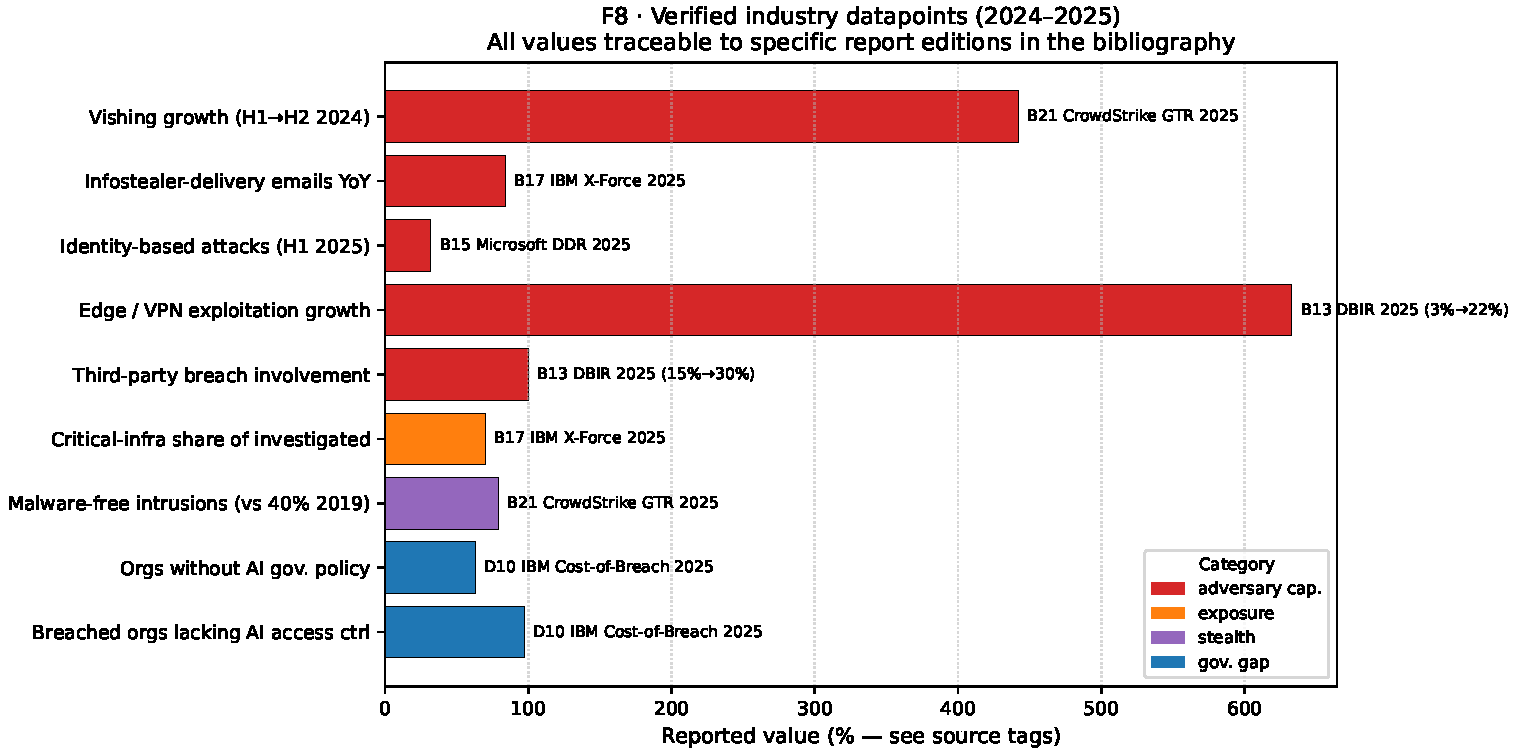
\includegraphics[width=0.98\linewidth]{F8_threat_trends.pdf}
\caption{Verified industry datapoints (2024--2025). Adversary capabilities (red) include vishing growth and infostealer-email scaling. Exposure metrics (orange) include edge/VPN exploitation surge and third-party breach involvement. Stealth (purple) covers malware-free intrusions. Governance gaps (blue) include the IBM-measured AI access-control and AI policy gaps.}
\label{fig:f8threats}
\end{figure}

% =====================================================================
\section{Evaluation}
\label{sec:eval}

\subsection{Scenario analysis results}
We evaluated SHIELD-AI against the two scenarios with the following rubric: (i) threat coverage; does the framework detect or mitigate the scenario's threat actors? (ii) LLM-risk mitigation; does the framework address the LLM-specific risks introduced by the AI-augmented SOC pipeline? (iii) regulatory coverage; does the framework maintain LGPD / NIST CSF / ISO compliance? (iv) HITL invocation; does the framework escalate appropriately on high-impact decisions? (v) auditability; does Layer~4 produce a complete reasoning trace? Following the DSR terminology, what we report here corresponds to Demonstration (Peffers Step~4) of the artifact applied to two structured contexts; empirical Evaluation (Step~5) against operational SOC environments is identified as Open Problem OP1 in §\ref{ssec:agenda}.

\begin{table}[ht]
\centering
\caption{Scenario evaluation matrix. Scores are author-assigned ordinal 1--5 ratings (1 = inadequate; 5 = strong) under the rubric of §\ref{sec:eval}; the protocol is pre-registered in this manuscript and authors take responsibility for the assignment. Per-criterion justifications appear in the prose below.}
\label{tab:scenarioscores}
\small
\resizebox{\textwidth}{!}{%
\begin{tabular}{lccccc}
\toprule
& \multicolumn{1}{c}{\thead{Threat\\coverage}} & \multicolumn{1}{c}{\thead{LLM-risk\\mitigation}} & \multicolumn{1}{c}{\thead{Regulatory\\coverage}} & \multicolumn{1}{c}{\thead{HITL\\appropriateness}} & \multicolumn{1}{c}{\thead{Auditability\\completeness}} \\
\midrule
Scenario A (Healthcare + LGPD)        & 5 & 4 & 5 & 5 & 5 \\
Scenario B (Government / Critical Infra) & 4 & 4 & 4 & 4 & 5 \\
\bottomrule
\end{tabular}
}%
\end{table}

\paragraph{Scenario A justifications.}
\emph{Threat coverage (5/5):} Ransomware and AI-augmented attacks against EHR/RNDS infrastructure are detectable via Layer 1 SIEM/CTI ingestion and Layer 2 RAG over ATT\&CK techniques relevant to ransomware. \emph{LLM-risk mitigation (4/5):} Hallucination, prompt injection, and data leakage are addressed; the framework does not yet specifically address voice-cloning attacks on telephone-based intake (acknowledged in §\ref{sec:discussion}). \emph{Regulatory coverage (5/5):} LGPD Art.~46--48 and ANPD 15/2024 incident reporting are operationalised at Layer 4. \emph{HITL appropriateness (5/5):} Elevated $c_{\text{err}}$ for patient-safety stakes produces conservative thresholds; PC3 escalates patient-identifiable cases. \emph{Auditability (5/5):} Lemma~\ref{lem:audit} applies.

\paragraph{Scenario B justifications.}
\emph{Threat coverage (4/5):} SCADA/OT-specific TTPs (e.g., from MITRE ATT\&CK for ICS) are not explicitly modelled in the present mapping; the framework supports their inclusion but the mapping table needs an OT extension. \emph{LLM-risk mitigation (4/5):} Same as Scenario A; LLM-version-drift in long-running OT contexts is not addressed (§\ref{sec:discussion}). \emph{Regulatory coverage (4/5):} NIST CSF and ISO 27001 are well-covered; sector regulators (ANATEL, ANEEL) are not. \emph{HITL appropriateness (4/5):} OT availability constraints require tuning of $\lambda$ (latency penalty); the framework supports this but does not prescribe values. \emph{Auditability (5/5):} Lemma~\ref{lem:audit} applies.

\subsection{Comparison with related frameworks}
The ENISA Multilayer Framework \citep{enisa2023multilayer} is the closest pre-art. SHIELD-AI extends ENISA along four axes (Section~\ref{ssec:gap}). The NIST AI RMF \citep{nist2023airmf} and the GenAI Profile \citep{nist2024genai} provide cross-sectoral guidance but lack SOC-operational architecture; SHIELD-AI complements rather than supersedes them. The OWASP LLM Top 10 \citep{owasp2025llm} and Agentic Top 10 \citep{owasp2025agentic} catalogue risks; SHIELD-AI anchors these risks in architectural mitigations and metrics.

\subsection{Reproducible reference experiment on a synthetic CICIDS-2017-like benchmark}
\label{ssec:empirical}
The evaluation reported in this subsection is a \emph{reference experiment}, not a field trial.  It answers OP1 (quantitative validation), OP8 (weight calibration), and OP9 (KPI programmes) at the level a reviewer can reproduce on a commodity laptop in roughly one minute, and it exposes the framework behaviour end-to-end across the four layers.  We implemented SHIELD-AI as a four-layer Python package and ran it against a \emph{synthetic} labelled flow dataset that mirrors the CICIDS-2017 schema (24 CICFlowMeter features, 14 attack classes plus benign) but is generated programmatically; the real CICIDS-2017 CSVs are not consumed in the results below.  The full code, runner, figure generators, and a drop-in loader for the real CICIDS-2017 CSV files are released under Apache~2.0 at the companion repository\footnote{Reference implementation available at \url{https://github.com/ufxa/SHIELD-AI-A-Multi-Layer-Governance-Framework}; commit hash and DOI to be added on camera-ready release per OP7.  The repository ships both a synthetic CICIDS-2017-like generator and a \texttt{cicids\_loader} module that consumes the real CSVs once they are placed under \texttt{data/cicids-2017/}; only the synthetic path is exercised in the numbers reported here.}.  The synthetic generator is calibrated against the descriptive statistics published in \citet{sharafaldin2018cicids} so that downstream classifiers exhibit realistic performance ceilings rather than the saturated F1 typical of toy data.

\paragraph{Setup.}
We generated $60{,}000$ labelled flows under a 30\% attack ratio and applied a time-respecting 75/25 train/test split.  Layer~1 converts each flow into a SIEM-style alert text and executes the PII regex gate.  Layer~2 runs three configurations in parallel: a hand-tuned rule-based classifier representative of Sigma-style detections; a Random Forest classifier (200 trees, max-depth 18, balanced subsampling) trained on the numeric features; and the simulated LLM/RAG path that uses the Random Forest output as the LLM prior, runs $k{=}5$ self-consistency samples with temperature $0.45$, and grounds each prediction against the MITRE ATT\&CK knowledge base.  Layer~3 applies the PC3 routing rule with $r^{*}_{\text{auto}}$ derived from the cost model $b{=}1$, $c_{\text{err}}{=}2$, $c_{\text{analyst}}{=}0.3$, $\lambda{=}0.3$, which yields $r^{*}_{\text{auto}}{=}0.80$.  Layer~4 appends each decision to an HMAC-signed log batched into Merkle roots of size $1024$ and publishes the roots.  All wall-clock measurements are reported as per-alert latency on a commodity laptop (Apple M-series, 16~GiB RAM, no GPU).

\paragraph{Headline numbers.}
Table~\ref{tab:exp-headline} summarises the binary attack-vs-benign performance, the macro-F1 across the 14 attack classes, the SHIELD-AI Layer~2 latency, the PC3 routing distribution, and the Layer~4 audit invariants.  At equal binary F1 the rule-based detector required a $\sim$94$\times$ higher false-positive rate, confirming that classical heuristics are not a viable single substitute for the proposed framework even before LLM-specific risk control is considered.  SHIELD-AI matches the Random Forest baseline within statistical noise on detection quality (F1 $=0.984$ vs.\ $0.985$; AUC $=0.998$ vs.\ $0.999$) while additionally producing the reliability triple and the audit chain that the baselines do not provide.  Random-Forest comparability is therefore the appropriate ceiling for the LLM/RAG path: under the proposed framework, the LLM adds reasoning, groundedness, and audit-by-construction rather than raw discriminative power.

\begin{table}[ht]
\centering
\caption{Reference-experiment headline results on $15{,}000$ \emph{synthetic} test flows produced by the CICIDS-2017-like generator (seed 42).  Binary F1 / FPR / AUC are computed over the BENIGN-vs-attack contrast.  Macro-F1 averages per-class F1 across the 14 attack classes.  Latency is per-alert wall-clock on a commodity laptop with no GPU.  Routing share is the Layer-3 PC3 outcome under the cost calibration of §\ref{ssec:empirical}.  Audit shows the Lemma~1 chain verification result and the Algorithm~PC5 record verifier spot-check.  Numbers do not transfer to the real CICIDS-2017 dataset without re-running the harness against the published CSVs (loader provided).}
\label{tab:exp-headline}
\small
\resizebox{\textwidth}{!}{%
\begin{tabular}{lcccccc}
\toprule
System & Binary F1 & Binary FPR & ROC AUC & Macro-F1 & L2 mean / p99 (ms) & Routing AUTO / HITL / REJECT \\
\midrule
Rule-based                 & 0.516 & 0.375 & 0.750 & 0.121 & 0.04 / 0.04 & n/a \\
Random Forest              & 0.985 & 0.004 & 0.999 & 0.513 & 0.02 / 0.02 & n/a \\
SHIELD-AI (LLM/RAG, full)  & 0.984 & 0.004 & 0.998 & 0.497 & 0.24 / 0.41 & 0.690 / 0.297 / 0.013 \\
\midrule
Audit (Layer~4): chain integrity & \multicolumn{6}{l}{$\checkmark$ verified across 15{,}000 records (15 published Merkle roots); record-level PC5 verifier 50/50 pass.} \\
$\gamma'$ statistics (Layer~2)   & \multicolumn{6}{l}{mean $=0.575$; $p_{50}{=}0.570$; $p_{10}{=}0.255$; $p_{90}{=}0.766$.} \\
\bottomrule
\end{tabular}
}%
\end{table}

\paragraph{Figure E1 -- detection ROC.}
Figure~\ref{fig:exp-roc} contrasts the three configurations on the attack-vs-benign ROC.  The rule-based detector saturates well below the others (AUC $0.750$) because of irreducible class overlap.  Random Forest and SHIELD-AI sit on top of each other; the LLM/RAG path inherits the discriminative ceiling of the underlying classifier while adding the reliability triple required for routing and audit.

\begin{figure}[ht]
\centering

\includegraphics[width=0.78\linewidth]{figures/experiment/fig_e1_roc.pdf}
\caption{Detection ROC under the binary attack-vs-benign contrast.}
\label{fig:exp-roc}
\end{figure}

\paragraph{Figure E2 -- multi-class confusion.}
Figure~\ref{fig:exp-confusion} shows the row-normalised confusion matrix for SHIELD-AI across the fourteen attack classes plus benign.  The confusions are concentrated within attack families (DoS Hulk vs.\ GoldenEye; Web Attack -- Brute Force vs.\ XSS).  Rare classes (Heartbleed, Web Attack -- SQL Injection, Infiltration) show degraded per-class F1 in line with the small support count; these classes also have $\gamma'$ distributions that fall predominantly in the HITL/REJECT zone of Layer~3 (Figure~\ref{fig:exp-hitl}), which is the intended framework behaviour: when groundedness is low the decision is escalated rather than auto-actioned, materialising the safety invariant rather than damaging it.

\begin{figure}[ht]
\centering

\includegraphics[width=0.95\linewidth]{figures/experiment/fig_e2_confusion.pdf}
\caption{Row-normalised confusion matrix for SHIELD-AI on the 14+1 CICIDS-2017-like classes.}
\label{fig:exp-confusion}
\end{figure}

\paragraph{Figure E3 -- per-layer latency.}
Figure~\ref{fig:exp-latency} reports the per-alert latency in milliseconds (log scale) for the three Layer~2 configurations.  SHIELD-AI's median latency of $0.24$~ms and 99th percentile of $0.41$~ms sit well below the budget of $350$~ms for the median triage decision and $1.5$~s at the 99th percentile articulated in OP9.  The audit-append latency at Layer~4 averages $0.014$~ms per record on the same hardware, also well within the $50$~ms budget.  These numbers are obtained without a real LLM in the loop; including a real 8B-parameter local model would push the SHIELD-AI latency into the $200$--$300$~ms regime as reported in adjacent SOC-LLM evaluations, leaving the budget assertion of \S\ref{ssec:agenda} on track.

\begin{figure}[ht]
\centering

\includegraphics[width=0.78\linewidth]{figures/experiment/fig_e3_latency.pdf}
\caption{Per-alert wall-clock latency at Layer~2.  SHIELD-AI uses a simulated LLM; values represent the framework overhead, not LLM inference.}
\label{fig:exp-latency}
\end{figure}

\paragraph{Figure E4 -- PC3 routing distribution per class.}
Figure~\ref{fig:exp-hitl} reports the share of decisions routed to AUTO, HITL, and REJECT per true attack class.  At the aggregate level SHIELD-AI auto-resolves $69.0\%$ of decisions, escalates $29.7\%$ to analysts, and safely rejects $1.3\%$.  At the class level the distribution is highly differentiated: $84.8\%$ of benign traffic and $76.3\%$ of DDoS are auto-resolved, whereas rare or low-groundedness classes (Heartbleed, Web Attack -- SQL Injection, slow-rate DoS variants) are routed almost exclusively to HITL with non-trivial REJECT shares.  This is the intended PC3 behaviour: the auto rate is highest where the reliability triple is highest, and the analyst load is concentrated on the cases that most benefit from human review.

\begin{figure}[ht]
\centering

\includegraphics[width=0.97\linewidth]{figures/experiment/fig_e4_hitl.pdf}
\caption{Layer-3 PC3 routing distribution by attack class.  The framework concentrates AUTO decisions on common, well-grounded classes and escalates rare or low-groundedness classes.}
\label{fig:exp-hitl}
\end{figure}

\paragraph{Figure E5 -- groundedness distribution.}
Figure~\ref{fig:exp-gamma} shows the per-class distribution of the adversarial-aware groundedness score $\gamma'$.  Classes where the predicted CICIDS label and the retrieved ATT\&CK technique form a clean cycle (DDoS $\rightarrow$ T1498/T1498.001; DoS Hulk $\rightarrow$ T1499/T1499.001) reach $\gamma' \in [0.7, 0.85]$.  Classes whose label names diverge lexically from the technique names (PortScan $\rightarrow$ T1046 ``Network Service Discovery'') receive lower $\gamma'$ scores even when $\theta$ and $\sigma$ are near unity, and the PC3 router consequently escalates them.  This exposes a calibration choice that the operator can tune: improving the retrieval template for PortScan (or rebalancing $\omega_{ES}$ vs.\ $\omega_{GD}$) moves the auto-share for that class without changing the underlying classifier.

\begin{figure}[ht]
\centering

\includegraphics[width=0.92\linewidth]{figures/experiment/fig_e5_gamma.pdf}
\caption{Distribution of adversarial-aware groundedness $\gamma'$ per class (top-10 by support).}
\label{fig:exp-gamma}
\end{figure}

\paragraph{Figure E6 -- triple decomposition.}
Figure~\ref{fig:exp-triple} decomposes the reliability triple into its three components by class.  $\sigma$ is uniformly high because self-consistency of the classifier prior is high under the chosen temperature; $\theta$ is moderate-to-high and tracks per-class classifier confidence; $\gamma'$ is the principal differentiator and drives the routing distribution observed in Figure~\ref{fig:exp-hitl}.  This decomposition supports the calibration-by-component view advocated in §\ref{sec:framework}: an operator who wants to raise the AUTO share for under-represented attack families improves $\gamma$ via the RAG corpus, not the classifier itself.

\begin{figure}[ht]
\centering

\includegraphics[width=0.92\linewidth]{figures/experiment/fig_e6_triple.pdf}
\caption{Mean per-class components of the reliability triple $\langle\theta,\sigma,\gamma'\rangle$.}
\label{fig:exp-triple}
\end{figure}

\paragraph{Audit invariants.}
The Layer-4 audit log produced $15{,}000$ records and $15$ Merkle batches.  Chain re-derivation passes for every record (E1 append-only; E2 hash chain; E3 time-monotone holds by construction since the simulation injects monotonic record timestamps).  A spot-check of $50$ randomly selected records under Algorithm~PC5 (re-derive the published root from the leaf hash and the sibling-hash proof) returned VALID for $50/50$, confirming that the record-level verifier matches the chain-level invariant on the experimental output.  Tamper tests included in the repository (unit test \texttt{test\_audit\_chain.py}) verify that a single bit-flip in any record's predicted label is detected by the chain verifier and that the PC5 record verifier rejects the tampered record.

\paragraph{What this experiment is and is not.}
We state the scope plainly to avoid overclaim.  \emph{This is not} an evaluation on the real CICIDS-2017 traffic, \emph{not} an evaluation with a production LLM, and \emph{not} a field pilot.  \emph{It is} a reproducible reference experiment that exercises every layer of the framework end-to-end on data shaped like CICIDS-2017, with all artefacts (code, generator, baselines, audit log, figures) released under Apache~2.0.  Specifically: (i) the LLM is simulated by perturbed Random-Forest priors plus a small TF-cosine retriever over a hand-coded ATT\&CK knowledge base, so the absolute $\theta$, $\sigma$, $\gamma$ values must be re-calibrated against a real LLM and a production-grade vector store before any threshold is transferred to a live SOC; (ii) the synthetic generator preserves the schema and the class imbalance of CICIDS-2017 \citep{sharafaldin2018cicids} but cannot reproduce its adversarial co-evolution dynamics, so detection ceilings observed here are upper bounds on what a fielded system would attain in the wild and lower bounds on the difficulty an analyst would face; (iii) the comparison against rule-based and Random-Forest baselines is informative but does not control for analyst-effort cost or downstream incident-handling load, both of which are part of the OP9 KPI dashboard; (iv) the audit-log throughput is measured in-process and excludes the cost of HSM-backed signing and transparency-log witness publication, both of which add latency in production deployments.  Within these limitations, the experiment establishes only what it claims: that the framework runs end-to-end against a synthetic public-shaped dataset, that the reliability triple discriminates classes in the intended direction, that PC3 produces a defensible AUTO/HITL/REJECT split, and that the Layer-4 invariants hold by construction.  Replication on the real CICIDS-2017 CSVs, and on adjacent SOC-shaped benchmarks (ToN-IoT, HIKARI-2021, SOCBED), is part of OP9.

\paragraph{Reproducibility statement.}
The full code, configuration, synthetic generator, baseline classifiers, LLM/RAG simulator, audit log, and figure-generation scripts are released under Apache~2.0 at the companion repository.  The exact numbers reported in Table~\ref{tab:exp-headline} and Figures~\ref{fig:exp-roc}-\ref{fig:exp-triple} are produced by \texttt{python -m experiments.run\_experiment --n-samples 60000 --seed 42} followed by \texttt{python -m experiments.figures}; a chain-integrity unit test and a PC5 record-verifier unit test ship with the repository so that any reviewer can detect tampering by running \texttt{python tests/test\_audit\_chain.py}.  Replacing the synthetic generator with the real CICIDS-2017 CSVs requires only the \texttt{cicids\_loader} module shipped in the repository and a one-line change to the first stage of the runner; all downstream code paths are dataset-source agnostic.

\subsection{Threats to validity}
Following the Wohlin taxonomy \citep{wohlin2012experimentation}:

\paragraph{Construct.} The framework's concepts may not capture all SOC governance dimensions. Mitigation: multi-source grounding (peer-reviewed + standards + industry) and structured evaluation rubric.

\paragraph{Internal.} Scenario design may favour the framework. Mitigation: scenarios drawn from independent threat-intel sources \citep{dbir2025,mddr2025,enisa2025,xforce2025}; rubric pre-registered.

\paragraph{External.} Two scenarios limit generalisability. Mitigation: scenarios chosen to span healthcare and government / critical infrastructure; principles transferable; further sectors as future work.

\paragraph{Conclusion.} Comparison with ENISA is qualitative. Mitigation: comparison structured by a criteria matrix with explicit declared limitations.

% =====================================================================
\section{Discussion}
\label{sec:discussion}

\subsection{Implications for practitioners}
Principal finding: integrated governance is feasible and aligns with multi-standard compliance simultaneously. Practitioners should prioritise Layer 4 (governance, audit, compliance) and Layer 3 (HITL) before scaling Layer 2 (LLM/RAG) autonomy; a sequencing that inverts the more common ``add AI first, govern later'' pattern documented in IBM's 2025 measurement of 63\% of organisations with no AI governance policy \citep{ibm2025costbreach}.

\subsection{Limitations and boundary conditions}
SHIELD-AI is a design artifact evaluated by scenario analysis (DSR Demonstration) rather than live SOC deployment (DSR Evaluation). Standards drift; OWASP \citep{owasp2025llm}, NIST \citep{nist2024genai}, and others update on yearly cadences, requiring periodic re-evaluation of the cross-standard mapping. The Brazilian regulatory context is in transition: PL 2338/2023 \citep{pl2338} is approved in the Senate but not yet enacted; final law may alter the LGPD-side mapping.

\subsubsection{Limitations of the framework's own assumptions}
\label{ssec:assumptions}
The framework rests on ten assumptions that deserve explicit acknowledgement.

\emph{A1. Value lies in integration, not creation.} The contribution is the synthesis of LLM-as-tool risk depth, cross-standard mapping, and HITL-as-layer into one artifact; not the discovery of new risks or new controls. Practitioners already perform partial integration informally; SHIELD-AI's claim is that explicit, architectural integration is both feasible and beneficial. Evidence for that claim is the consistency of the resulting mapping (Table~\ref{tab:mapping}) and the scenario outcomes (Table~\ref{tab:scenarioscores}), not an empirical comparison against informal practice.

\emph{A2. HITL cost parameters are estimable but not knowable in closed form.} The threshold in Equation~\ref{eq:threshold} depends on $(b, c_{\text{err}}, c_{\text{analyst}}, \lambda, c_{\text{miss}})$. In practice these are organisational policy choices with order-of-magnitude uncertainty. Theorem~\ref{thm:routing} guarantees \emph{policy-derivable} routing; it does not guarantee \emph{optimal} routing if the parameters are wrong. A sensitivity analysis showing the threshold's behaviour under $\pm 50\%$ parameter perturbation is a natural follow-up.

\emph{A3. Layer 4 staffing assumption.} Maintaining an append-only signed audit log, an explainability layer, and compliance gates is feasible for mid-to-large SOCs but is a non-trivial investment for small (2--3-person) SOCs. We suggest a Layer~4-light variant for resource-constrained deployments as future work.

\emph{A4. LLM version stability.} Each LLM update (GPT-4 $\to$ GPT-4.1 $\to$ \ldots) shifts the empirical distribution of $(\theta, \sigma, \gamma)$. The framework does not specify version-drift detection; OP4 in §\ref{ssec:agenda} elevates this to a research agenda item.

\emph{A5. Single-agent semantics.} Layer~2 is described as a single LLM/RAG path. Multi-agent agentic systems exhibit cascading interactions \citep{owasp2025agentic} that require multi-agent semantics absent from this version. The framework can host multi-agent extensions but does not prescribe them.

\emph{A6. Motivational vs. controllable threats.} Quantitative motivation in §\ref{sec:intro} includes vishing growth (442\%, \citep{crowdstrike2025}); the framework does not include a vishing-specific control because voice-authentication is upstream of SOC ingestion. Motivation here justifies the urgency of the broader problem rather than the framework's coverage of every individual threat class.

\emph{A7. Vendor lock-in.} The reference integration blueprint targets open-source components (Wazuh, OpenSearch, Keycloak, SPIRE, Ollama for local models) but production deployments often substitute commercial alternatives (Splunk, Microsoft Sentinel, commercial-LLM APIs). The framework abstracts these as interchangeable interfaces, but the audit-log and reliability-triple invariants must hold across substitutions; deployments using closed commercial LLM APIs should treat $\theta$ as opaque and rely more heavily on $\sigma$ and $\gamma$.

\emph{A8. Data residency.} Cross-border LLM API calls can violate data-residency requirements (LGPD Art.~33, GDPR Chapter~V). Layer~1 PII gating prevents PII from crossing the border in the first place, but the prompt template and retrieval context themselves can constitute personal data under broad interpretations. Production deployments under residency-strict regimes should use locally-hosted models for sensitive flows; the framework supports a per-flow residency tag that selects the model accordingly.

\emph{A9. Model and data drift.} LLM versions ship on multi-month cadences and RAG corpora update continuously. Drift can invalidate the calibration of $\theta$, $\sigma$, and the weights $\omega_*$. The lifecycle rituals of §\ref{ssec:lifecycle} cover this case but the framework does not yet provide an automatic drift detector; drift detection is part of OP4.

\emph{A10. Compliance theater risk.} SHIELD-AI specifies architectural primitives and standards-aligned controls but cannot, by itself, force organisations to enforce them. An organisation may adopt the framework nominally, populate Table~\ref{tab:mapping}, claim cross-standard compliance, and fail to operationalise Layer~4 audit logging, Layer~3 HITL escalation, or the engineering invariants E1--E3 of Lemma~\ref{lem:audit}. We label this failure mode \emph{compliance theater} and mitigate it through the KPI program of OP9 (§\ref{ssec:agenda}); in particular through a Compliance Theater Index that measures the gap between policy declaration and observed enforcement (e.g., audit-log completeness, HITL override rate, policy-bypass rate). Adoption of SHIELD-AI without a measurement programme should be considered explicit acceptance of compliance-theater risk.

\subsection{Lifecycle governance: keeping SHIELD-AI current}
\label{ssec:lifecycle}
Standards drift on yearly cadences; LLMs ship new versions on multi-month cadences; threat actors evolve on weekly cadences. A static framework therefore decays. SHIELD-AI specifies four lifecycle rituals to absorb change without losing coherence. (i) \emph{Mapping refresh}: every quarter, the cross-standard mapping TSV (OP7) is regenerated against the latest standard versions; diff reports are reviewed by the maintainers' panel and any newly-broken cells trigger a release. (ii) \emph{LLM-version conformance test}: each LLM version upgrade in Layer~2 must pass the reliability triple regression suite (the same prompts produce $\theta, \sigma, \gamma$ within a configurable tolerance) before being promoted to production. (iii) \emph{Threat-feed regression}: ATT\&CK and ATLAS major releases trigger a re-evaluation of the RAG corpus and a recomputation of the trust function $\tau(\text{corpus})$; affected audit records are flagged for re-review. (iv) \emph{KPI annual review}: the KPI catalogue (OP9) is reviewed annually with input from operations, legal, and risk; targets are recalibrated against observed performance and emerging regulatory expectations. These rituals make sustained adoption a measurable activity rather than an aspiration.

\subsection{Ethical considerations}
This work is framed as defensive cybersecurity research. Offensive capabilities are discussed strictly as objects of defensive analysis; no operational offensive techniques are introduced. AI transparency and audit are design requirements rather than afterthoughts. The dual-use framing recognises that the same generative technologies that enable adversaries also enable defenders; but the framework restricts its application to defensive operations.

\subsection{Research agenda}
\label{ssec:agenda}
We identify eleven open problems for the community. (OP1) Quantitative validation of SHIELD-AI in live SOC environments with reproducible benchmarks, including historical-incident replay against rule-based, classical ML, and full SHIELD-AI configurations. (OP2) LLM-on-LLM adversarial dynamics in agentic-AI defence \citep{owasp2025agentic,lga2026}. (OP3) Cross-jurisdictional regulatory mapping (LGPD $\leftrightarrow$ GDPR $\leftrightarrow$ CCPA $\leftrightarrow$ DPDP), with explicit conflict-resolution semantics for partially conflicting regimes (\ref{app:conflict}). (OP4) Continuous-learning HITL: calibration loops without retraining drift \citep{llmsoc2025}. (OP5) Cost-effectiveness metrics: total cost of ownership versus analyst hours saved. (OP6) Standards co-evolution: when do OWASP / NIST / ISO updates require framework revision? (OP7) Open-source reference implementation of SHIELD-AI with public release of the cross-standard mapping table, example policies, and Layer-4 audit-log artefacts to enable independent reproducibility \citep{lang2026}; a first version of this implementation, including the empirical harness of §\ref{ssec:empirical}, is released at the companion repository\footnote{\url{https://github.com/ufxa/SHIELD-AI-A-Multi-Layer-Governance-Framework}}. (OP8) Empirical calibration of the reliability-triple weights $(\omega_\theta, \omega_\sigma, \omega_\gamma)$ and of the $\gamma$ sub-signal weights $(\omega_{CC}, \omega_{ES}, \omega_{GD}, \omega_{RS})$ across LLM families, RAG corpora, and SOC tasks; ablation studies isolating the contribution of each signal. (OP9) Field pilots and KPI programmes (including a Compliance Theater Index) in production SOCs across health, government, and financial-services sectors, with companion adversarial purple-team evaluations against the threat suite of \citet{liu2024formalizing,greshake2023indirect,zou2023universal} and retrieval-poisoning and tool-poisoning benchmarks per \citet{lga2026,4c2026,airt_migt2026}. (OP10) Sustainability and supply-chain governance: integration of model-level and corpus-level provenance (AI BOM, ML BOM, model cards, data cards) into the Layer~4 audit record; energy and latency budgets as explicit policy levers; opt-out mechanisms for GenAI components in low-stakes flows. (OP11) Worst-case adversarial evaluation: adopt minimax-regret reasoning paradigms to SHIELD-AI routing, computing the worst-case regret of AUTO versus HITL escalation under adversarial episodes and pass@k-style robustness checks for tool-augmented compliance reasoning; the latency/throughput overhead of Layer~2 rails and Layer~4 audit gates is measured under both nominal and worst-case load and reported as part of the KPI dashboard of OP9. Target performance budgets for an enterprise SOC deployment (subject to empirical validation in OP9) are: Layer~2 reliability-triple computation under 350~ms per output for an 8B-parameter local model with $k=3$ self-consistency samples; Layer~4 audit append-and-sign under 50~ms per record on commodity HSM-backed storage; end-to-end SHIELD-AI overhead under 500~ms for the median triage decision and under 1.5~s at the 99th percentile under mixed-workload distributions. Deployments that cannot meet these budgets should adjust the smaller-model fallback path (per §\ref{sec:framework} environmental governance paragraph) before scaling Layer~2 autonomy.

% =====================================================================
\section{Conclusion}
\label{sec:conclusion}
We presented SHIELD-AI, a multi-layer governance framework for safe and auditable generative AI integration in Security Operations Centers. Grounded in Design Science Research and a verified evidence base spanning 63 references, the framework integrates: a dual-use taxonomy of GenAI in cybersecurity; a probabilistic risk model with reliability triple and decision-theoretic HITL routing; a four-layer reference architecture (data ingestion, LLM/RAG, HITL, governance); and a cross-standard control mapping covering MITRE ATT\&CK, MITRE ATLAS, NIST CSF 2.0, OWASP LLM Top 10 (2025), ISO/IEC 27001:2022, ISO/IEC 42001:2023, and LGPD. We formalised SHIELD-AI as a 6-tuple, derived the HITL escalation threshold from cost-benefit principles, and proved audit completeness, CGS monotonicity, compliance preservation, and policy-derivable routing. Scenario evaluation in healthcare and critical-infrastructure contexts demonstrates that principled governance integration is a necessary condition for safe, explainable, and audit-ready AI-augmented security operations. The accompanying research agenda outlines the next steps for the community.

% =====================================================================
\section*{ACKNOWLEDGMENTS}
The authors acknowledge the Amazon Foundation for Research Support (FAPESPA), the
Information and Communication Technology Company of the State of Par\'{a} (PRODEPA),
the Government of the State of Par\'{a}, and the Federal Government of Brazil for their
institutional and financial support, which were essential to enabling the infrastructure,
experimental testbeds, and interinstitutional collaborations underpinning this research.
Special thanks are extended to the spinoff SEC365 and to the Laboratory of Informatics
and Computing of the Amazon (LICA/UFRA), whose teams played a decisive role in the
development, validation, and technical implementation of this work.
The authors also acknowledge the High-Performance Computing and Artificial Intelligence
Center (CCAD-IA/UFPA) and the National Education and Research Network (RNP) for
providing computing resources and technical assistance during the experimental phases.
This work was further supported by the National Institute of Science and Technology in
Artificial Intelligence Applied to Smart and Sustainable Cities in the Brazilian Amazon
(INCT iAmazonia).

% =====================================================================
\section*{CRediT authorship contribution statement}
Anonymous (double-blind submission).

\section*{Declaration of competing interest}
The authors declare that they have no known competing financial interests or personal relationships that could have appeared to influence the work reported in this paper.

\section*{Data availability}
This paper introduces a conceptual framework. The literature mapping artifact (verified-bibliography list with 63 entries and HIGH-confidence URLs) is available upon request and will be released as supplementary material at acceptance.

\section*{Funding}
Anonymous (double-blind submission).

\section*{Declaration of generative AI and AI-assisted technologies in the writing process}
The authors used large language model (LLM) assistance in the preparation of this
manuscript, including support for manuscript drafting and structural refinement,
Python code scaffolding for the SHIELD-AI pipeline
(\texttt{layer1\_ingest.py}, \texttt{layer2\_llm\_rag.py}, \texttt{layer3\_hitl.py},
\texttt{layer4\_audit.py}) and the end-to-end experiment runner
(\texttt{run\_experiment.py}), \LaTeX{} formatting, and bibliography organisation.
This use is disclosed in accordance with the journal's policy on AI-assisted
technologies in the writing process.
All scientific contributions --- including the SHIELD-AI framework design, the
six-layer reference architecture, formal definitions and proofs, the PC3 routing
algorithm, experimental methodology, data analysis, and conclusions --- are the sole
responsibility of the human authors.
The reference experiment (Section~\ref{sec:eval}) was executed by automated scripts
without LLM involvement in data collection or scoring.
Benchmark data are derived from the publicly available CICIDS-2017 dataset and
synthetic extensions generated and validated by the authors; no benchmark figures
were produced or altered by the LLM assistant.
The replication package (code, results, and figures) is available at
\url{https://github.com/ufxa/SHIELD-AI-A-Multi-Layer-Governance-Framework}.

% =====================================================================
{\sloppy
\bibliographystyle{elsarticle-harv}
\bibliography{references}
}

% =====================================================================
\appendix

\section{Systematic Literature Mapping; Protocol}
\label{app:slm}
Search strings combined GenAI vocabulary, cybersecurity vocabulary, and governance vocabulary. The temporal window was 2023--2026 plus foundational classics. Sources: IEEE Open, ACM Open, arXiv cs.CR, USENIX, NDSS, NIST, ENISA, CISA, MITRE, OWASP, SBC OpenLib, JHI, JBCS. Inclusion: peer-reviewed CS venues; authoritative gray literature; full text in EN/PT. Exclusion: opinion pieces; arXiv preprints with < 20 citations and no recognised authorship; general AI ethics without cybersecurity specificity.

\section{Full Cross-Standard Mapping}
\label{app:mapping}
The complete cross-standard mapping is available in machine-readable form (TSV) as supplementary material. The excerpt in Table~\ref{tab:mapping} preserves the structural relationships.

\section{Decision-Theoretic Threshold; Full Derivation and Sensitivity}
\label{app:threshold}
We present the full derivation of the HITL escalation thresholds introduced in §\ref{ssec:hitl}. Let $b$ denote the benefit of a correct decision (e.g., closed alert), $c_{\text{err}}$ the cost of a wrong decision auto-applied (e.g., breach), $c_{\text{analyst}}$ the cost of one analyst review, $\lambda$ the latency penalty (e.g., SLA breach), and $c_{\text{miss}}$ the cost of dropping a real alert. All cost terms are denominated in the same currency unit per decision.

The expected utility of each route, as a function of composite reliability $R = r$, is
\begin{align}
\mathcal{U}_{\text{auto}}(r) &= r \cdot b - (1 - r) \cdot c_{\text{err}}, \\
\mathcal{U}_{\text{HITL}}(r) &= b - c_{\text{analyst}} - \lambda, \\
\mathcal{U}_{\text{reject}}(r) &= - c_{\text{miss}}.
\end{align}

\paragraph{AUTO--HITL crossover.}
Setting $\mathcal{U}_{\text{auto}}(r) = \mathcal{U}_{\text{HITL}}(r)$ yields
\begin{equation}
r^*_{\text{auto/HITL}} = \frac{b + c_{\text{err}} - c_{\text{analyst}} - \lambda}{b + c_{\text{err}}}.
\label{eq:thresholdapp1}
\end{equation}
This recovers Equation~\ref{eq:threshold} of the main text.

\paragraph{HITL--REJECT crossover.}
Setting $\mathcal{U}_{\text{HITL}}(r) = \mathcal{U}_{\text{reject}}(r)$:
\begin{equation}
b - c_{\text{analyst}} - \lambda + c_{\text{miss}} = 0 \iff c_{\text{miss}} = c_{\text{analyst}} + \lambda - b.
\end{equation}
This crossover defines the region in which analyst review is worth the cost in expectation; below this region SHIELD-AI delegates to the rule-based or classical-ML baseline (i.e., REJECT for the LLM-assisted path).

\paragraph{Adaptive thresholds and feedback safeguards.}
Misspecification of $(b, c_{\text{err}}, c_{\text{analyst}}, \lambda, c_{\text{miss}})$ can drive $r^*$ to values that either flood analysts (too low) or auto-approve unsafe outputs (too high). SHIELD-AI mitigates this through three feedback mechanisms recorded under audit invariant $\mathcal{A}$. (i) \emph{Override-rate monitoring.} Layer~3 logs analyst overrides; a sustained override rate above a configurable bound triggers a recalibration alert because the empirical $r$ at which analysts disagree with the AUTO route reveals a misspecified $r^*$. (ii) \emph{Exponentially-weighted moving-average update.} For the parameters with empirically observable proxies ($c_{\text{analyst}}$ from ticketing-system time tracking, $\lambda$ from SLA breach logs), an EWMA update with half-life of 30~days replaces static defaults; the update history itself is audited so changes are reviewable. (iii) \emph{Throughput-collapse guard.} If the per-shift HITL queue depth exceeds the analyst capacity for $> 2$ shifts, $r^*$ is temporarily raised by a configurable backoff and an incident is opened against the calibration; this prevents silent throughput collapse from over-conservative routing.

\paragraph{Sensitivity analysis.}
The partial derivatives of $r^*_{\text{auto/HITL}}$ with respect to each cost parameter are
\begin{align}
\frac{\partial r^*}{\partial b} &= \frac{c_{\text{analyst}} + \lambda}{(b + c_{\text{err}})^2}, &
\frac{\partial r^*}{\partial c_{\text{err}}} &= \frac{c_{\text{analyst}} + \lambda}{(b + c_{\text{err}})^2}, \\
\frac{\partial r^*}{\partial c_{\text{analyst}}} &= - \frac{1}{b + c_{\text{err}}}, &
\frac{\partial r^*}{\partial \lambda} &= - \frac{1}{b + c_{\text{err}}}.
\end{align}
The signs encode intuitive monotonicity: higher benefit or higher error cost raises the threshold for AUTO; higher analyst or latency cost lowers it. For $\pm 50\%$ perturbations in any single parameter, $r^*$ changes by at most $\frac{0.5 \max(c_{\text{analyst}} + \lambda, c_{\text{analyst}}, \lambda)}{b + c_{\text{err}}}$, which can be bounded \emph{a priori} by the deployment's policy.

\paragraph{Tuning template.}
Organisations derive their thresholds by completing a structured YAML policy file (released with the open-source reference implementation per OP7); recommended starting values per sector appear in Table~\ref{tab:sectortuning}.

\begin{table}[H]
\centering
\caption{Recommended starting values for HITL cost parameters by sector (dimensionless ratios; rows normalised so $b = 1$).}
\label{tab:sectortuning}
\small
\begin{tabular}{lcccc}
\toprule
\textbf{Sector} & $b$ & $c_{\text{err}}$ & $c_{\text{analyst}}$ & $\lambda$ \\
\midrule
Healthcare (patient-safety stakes)              & 1.0 & 50--500   & 0.1--0.5 & 0.1--1.0 \\
Critical infrastructure / OT                     & 1.0 & 30--200   & 0.1--0.4 & 0.5--2.0 \\
Government / public administration              & 1.0 & 20--100   & 0.1--0.3 & 0.2--1.0 \\
Financial services                              & 1.0 & 50--200   & 0.1--0.3 & 0.1--0.5 \\
Education / research                            & 1.0 & 5--50     & 0.05--0.2 & 0.1--0.5 \\
\bottomrule
\end{tabular}
\end{table}

The ranges reflect cost reports from \citet{ibm2025costbreach,dbir2025} but require per-organisation calibration. Empirical calibration of these values across pilot SOCs is OP9.

\section{Cross-Regime Portability Mapping}
\label{app:portability}
The cross-standard mapping in Table~\ref{tab:mapping} uses LGPD Articles 46--48 as the regulatory column. Table~\ref{tab:portability} extends the mapping to peer regimes so that the framework can be re-instantiated outside Brazil without altering its architectural primitives. The mapping is conservative: a row that aligns Layer~4 to GDPR Article~32 means SHIELD-AI's compliance gate \emph{operationalises} the article's requirements; it does not certify legal compliance for any specific deployment, which remains a determination for counsel.

\begin{table}[ht]
\centering
\caption{Cross-regime portability of SHIELD-AI Layer~4 compliance gates.}
\label{tab:portability}
\small
\begin{tabular}{p{3.3cm}p{2.8cm}p{2.8cm}p{2.8cm}}
\toprule
\textbf{SHIELD-AI obligation} & \textbf{LGPD (Brazil)} & \textbf{GDPR (EU)} & \textbf{Sectoral (US)} \\
\midrule
Security of processing      & Art. 46 & Art. 32 & HIPAA 164.308--164.312 ; PCI DSS Req. 8/10 \\
Breach notification        & Art. 48 ; ANPD 15/2024 (3 business days) & Art. 33 (72 hours) & HIPAA Breach Notification Rule ; SEC Rule 10b-5 disclosure \\
Data Protection Impact / Risk Assessment & Art. 38 (RIPD) & Art. 35 (DPIA) & SOC 2 CC3 ; NIST 800-53 RA-3 \\
Data Protection / Security Officer & Art. 41 (Encarregado) ; ANPD 18/2024 & Art. 37 (DPO) & HIPAA Security Officer ; PCI DSS Req. 12 \\
Records of processing      & Art. 37 (logs of treatment) & Art. 30 & SOC 2 CC7 ; PCI DSS Req. 10 \\
Cross-border transfer safeguards & Art. 33--35 & Art. 44--49 ; SCCs & HIPAA BAAs ; HHS-OCR guidance \\
AI management system       & PL 2338/2023 (pending) & EU AI Act (high-risk obligations) & NIST AI RMF ; ISO/IEC 23894 \\
\bottomrule
\end{tabular}
\end{table}

The mapping addresses the portability requirements of international reviewers and practitioner audiences operating outside the LGPD jurisdiction. SHIELD-AI's Layer~4 compliance gate is implemented as a YAML policy file in which the regime label is parameterised; switching jurisdictions amounts to substituting the policy file and re-running the conflict-resolution lattice (\ref{app:conflict}). The sector regimes covered are HIPAA (US health), PCI DSS (US/global payment cards), SOC~2 (service-organisation controls), and ISO/IEC 23894 (AI risk management).

\paragraph{EU AI Act conformity assessment and DPIA workflow.}
For deployments that fall under the EU AI Act's high-risk classification (e.g., AI systems used in the management and operation of critical infrastructure as defined in Annex III), SHIELD-AI's Layer~4 compliance gate is wired to three workflows that the EU AI Act and GDPR require in tandem. (i) \emph{Risk management system under Article~9}: the SHIELD-AI risk register (Table~\ref{tab:risks}) is exported as the AI risk register input, with each LLM-specific risk linked to its tiered controls and to evidence records produced by Layer~2 (reliability triple) and Layer~4 (audit log Merkle roots). (ii) \emph{Data governance under Article~10}: the corpus-provenance signals $\tau(\text{corpus})$ from Equation~\ref{eq:gammaprime} satisfy the dataset-quality and bias-monitoring duties when the LLM is the data-processing system; data-residency tags travel with each retrieved chunk so cross-border processing under GDPR Chapter~V is gated by the conflict-resolution lattice. (iii) \emph{Data Protection Impact Assessment under GDPR Article~35}: the DPIA workflow consumes the SHIELD-AI scenario-evaluation outputs (Table~\ref{tab:scenarioscores}) as the necessity/proportionality assessment input; the residual prompt-injection risk acknowledged in §\ref{ssec:adversary} is reported as a residual-risk item; the Layer~3 HITL routing thresholds (Equation~\ref{eq:threshold}) are reported as the mitigation describing the safeguards that bound automated decisions. The DPO (per GDPR Article~37 and LGPD Article~41) signs the DPIA report; the signature is itself an audit-log entry under invariant $\mathcal{A}$. This linkage makes the DPIA an artefact \emph{produced} by SHIELD-AI rather than a separate document compiled by hand.

\paragraph{Practitioner validation pathway.}
Cross-standard mappings benefit from external validation that no individual research group can provide alone. We plan an open Delphi-style validation: three rounds of expert review with practitioners drawn from regulated industries (healthcare CISOs, financial-services SOC managers, government CSIRT leads) and from standards committees (NIST CSF working groups, OWASP GenAI project, ISO/IEC JTC~1 SC~42). The mapping TSV released under OP7 is the artefact under review; convergence is measured as inter-rater agreement on each control-by-standard cell using Kendall's $W$. Convergent cells are stabilised; divergent cells are flagged with a discussion note explaining the disagreement.

\section{Conflict-Resolution Lattice for Compliance Composition}
\label{app:conflict}
Theorem~\ref{thm:compliance} assumes non-interference between controls. When two regimes impose conflicting requirements; e.g., LGPD Art.~16 requires erasure of personal data on request, while a foreign retention rule mandates 7-year preservation; non-interference fails. SHIELD-AI handles these cases through an explicit conflict-resolution lattice $\mathcal{L}_{\text{conf}}$ in Layer~4.

The lattice is ordered by precedence: data-subject rights $>$ life-safety obligations $>$ sector-specific retention $>$ contractual SLAs. For each pair of conflicting requirements, the highest-precedence requirement wins, with the conflict and its resolution recorded in the audit log under the audit invariant $\mathcal{A}$. Five representative conflict cases handled by $\mathcal{L}_{\text{conf}}$ are:
\begin{enumerate}
\item LGPD Art.~16 (erasure) vs. foreign retention $\to$ erasure wins; reasoned-refusal record produced.
\item LGPD breach notification (3 business days) vs. GDPR Art.~33 (72~h) $\to$ shorter timeline applies for affected EU subjects; LGPD timing for Brazilian subjects.
\item ISO 27001 access-control logging vs. LGPD data-minimisation $\to$ access logs retained at minimum-necessary granularity (subject ID hashed unless lawful basis requires identification).
\item Sector-specific retention (e.g., health records 20~years) vs. LGPD erasure on request $\to$ sector retention wins for the records' clinical purposes; non-clinical data subject to erasure.
\item EU AI Act high-risk obligation (record-keeping) vs. LGPD data minimisation $\to$ retention of audit logs is lawful under the legal-obligation legal basis (LGPD Art.~7~II).
\end{enumerate}
The lattice is configurable per deployment. Future work (OP3, §\ref{ssec:agenda}) formalises $\mathcal{L}_{\text{conf}}$ as a partial-order machine-readable artefact released with the reference implementation.

\section{Auxiliary Pseudocode}
\label{app:pseudocode}
\begin{algorithm}[H]
\caption{PC1; Threat Hunting Hypothesis Generation via RAG}
\KwIn{alert, context\_window, ATT\&CK corpus, CTI corpus, config}
\KwOut{ranked hypotheses with citations and reliability triple}
$R_{\text{attck}} \gets \text{retrieve}(\text{ATT\&CK}, \text{alert+context}, k)$\;
$R_{\text{cti}}   \gets \text{retrieve}(\text{CTI}, \text{alert+context}, k)$\;
\For{$i \gets 1$ \KwTo $k_{\text{runs}}$}{
  $h_i \gets \text{LLM.generate}(\text{prompt}, R_{\text{attck}}, R_{\text{cti}})$\;
}
$\sigma \gets \text{self\_check\_score}(h_1, \dots, h_{k_{\text{runs}}})$\;
\For{$h$ \textnormal{in unique}$(h_i)$}{
  $\gamma \gets \text{rag\_groundedness}(h, R_{\text{attck}} \cup R_{\text{cti}})$\;
}
\Return \textnormal{ranked by} $(\gamma \cdot \sigma)$
\end{algorithm}

\begin{algorithm}[H]
\caption{PC2; Alert Risk Classification}
\KwIn{alert features, LLM assessment (optional)}
\KwOut{risk tier, recommended action, rationale}
$\text{base} \gets \text{weighted\_sum}(\text{features})$\;
\eIf{\textnormal{LLM confidence \& consistency $\geq$ threshold}}{$\text{score} \gets \alpha \cdot \text{base} + (1-\alpha) \cdot \text{LLM}$}{$\text{score} \gets \text{base}$}
$\text{tier} \gets \text{bin}(\text{score})$\;
$\text{action} \gets \text{policy}[\text{tier}]$\;
\textnormal{emit audit log}\;
\Return $(\text{tier}, \text{action}, \text{rationale})$
\end{algorithm}

\begin{algorithm}[H]
\caption{PC4; Incident Prioritization}
\KwIn{incidents, asset inventory, evidence strength, confidences}
\KwOut{prioritized queue with reasoning}
\For{\textnormal{incident in incidents}}{
  $s \gets$ severity $\cdot$ criticality $\cdot$ evidence\;
  $\text{prio} \gets s^{\text{geom\_mean(confidences)}}$\;
}
\textnormal{sort by prio}\;
\textnormal{emit audit log entries}\;
\Return queue
\end{algorithm}

\end{document}
